\documentclass[a4paper]{report}
\usepackage[group-separator={,},group-minimum-digits={3}]{siunitx}
\usepackage[utf8]{inputenc}
\usepackage[dvipsnames]{xcolor}
\usepackage{tcolorbox}
\usepackage{multicol}
\usepackage{lipsum}
\usepackage[margin=0.2in]{geometry}
\usepackage{xstring}
\usepackage{xifthen}
\usepackage[dvipsnames]{xcolor}
\usepackage{setspace}
\usepackage{amsmath}
\usepackage{enumitem}
\pagenumbering{gobble}
\setlength{\columnsep}{1.5cm}
\setlength{\columnseprule}{0.2pt}
\usepackage{hyperref}
\usepackage[none]{hyphenat}
\usepackage{graphicx}
\usepackage{etoolbox}
\usepackage{titlepic}
\usepackage[super]{nth}
\usepackage{setspace}
\usepackage{CJKutf8}
\usepackage[document]{ragged2e}

\hypersetup{
    colorlinks,
    citecolor=black,
    filecolor=black,
    linkcolor=black,
    urlcolor=black
}

\usepackage[default]{sourcesanspro}
\usepackage[T1]{fontenc}

\makeatletter
\def\@makechapterhead#1{%
  %\vspace*{5\p@}%
  {\parindent \z@ \raggedleft \normalfont
    \ifnum \c@secnumdepth >\m@ne
        \large\bfseries #1
        \par\nobreak
%        \vskip 10\p@
        \rule{\columnwidth}{.1pt}%
%        \vskip 10\p@
    \fi
    \interlinepenalty\@M
%    \large \bfseries \MakeUppercase{#1}\par\nobreak
%    \vskip 5\p@
  }}
\makeatother


\newcommand{\blitzloss}{\textbf{\textcolor{Magenta}{Blitz Loss}}}
\newcommand{\lostblitz}{\textbf{\textcolor{Magenta}{lost Blitz}}}

\newcommand{\blitzwin}{\textbf{\textcolor{OliveGreen}{Blitz Win}}}
\newcommand{\wonblitz}{\textbf{\textcolor{OliveGreen}{won Blitz}}}

\usepackage{enumitem}
\setitemize{noitemsep,topsep=0pt,parsep=0pt,partopsep=0pt}
\usepackage{graphicx}
\ifthenelse{%
        \equal{\blitzresult}{win}
    }{%
        \title{FFX Any\% - \blitzwin}
    }{%
        \ifthenelse{%
            \equal{\blitzresult}{loss}
        }{%
            \title{FFX Any\% - \blitzloss}
        }{%
            \ifthenelse
            }{}
        }
    }
\author{Mr.Tyton}
\titlepic{
\includegraphics[width=\textwidth]{final_fantasy_x_logo_by_eldi13_d4204zv}}
\begin{document}
\singlespacing
\maketitle
\tableofcontents

\makeatletter
\patchcmd{\chapter}{\if@openright\cleardoublepage\else\clearpage\fi}{}{}{}
\makeatother

\newenvironment{battle}[2][]{\begin{tcolorbox}[title=\begin{center}\MakeUppercase{#2} \ifthenelse{\isempty{#1}}{}{- \num{#1} HP}\end{center},colbacktitle=red!50!white,colframe=red!55,coltitle=black]}{\end{tcolorbox}}

\newenvironment{shop}[1]{\begin{tcolorbox}[title=\begin{center}SHOP\, #1 GIL\end{center},colbacktitle=blue!50!white,coltitle=black,colframe=blue!50!white]}{\end{tcolorbox}}

\newenvironment{spheregrid}[1][]{\begin{tcolorbox}[title=\begin{center}SPHERE GRID\ifthenelse{\isempty{#1}}{}{ - #1}\end{center},colbacktitle=purple!50!white,colframe=purple!55,coltitle=black]}{\end{tcolorbox}}

\newenvironment{encounters}{\begin{tcolorbox}[title=\begin{center}ENCOUNTERS\end{center},colbacktitle=VioletRed!50!white,colframe=VioletRed!55,coltitle=black]}{\end{tcolorbox}}

\newenvironment{trial}{\begin{tcolorbox}[title=\begin{center}CLOISTER OF TRIALS\end{center},colbacktitle=Bittersweet!50!white,colframe=Bittersweet!55,coltitle=black]}{\end{tcolorbox}}

\newenvironment{blitzball}{\begin{tcolorbox}[title=\begin{center}BLITZBALL\end{center},colbacktitle=Maroon!50!white,coltitle=black,colframe=Maroon!50!white]}{\end{tcolorbox}}

\newenvironment{equip}{\begin{tcolorbox}[title=\begin{center}EQUIPMENT\end{center},colbacktitle=Gray!50!white,coltitle=black,colframe=Gray!50!white]}{\end{tcolorbox}}

\newcommand{\link}[2]{\href{#1}{\textcolor{blue}{\underline{#2}}}}

\newcommand{\save}{\textbf{Touch the Save Sphere}}

\newcommand{\pickup}[1]{open the chest for the \textbf{#1}}

\newcommand{\sd}{\textbf{SD}}

\newcommand{\cs}[1][]{\textbf{CS}%
    \ifthenelse{\isempty{#1}}{}{ (#1)}%
}

\newcommand{\skippablecs}[1][]{\textbf{Skippable CS}%
    \ifthenelse{\isempty{#1}}{}{ (#1)}%
}

\newcommand{\fmv}[1][]{\textbf{FMV}%
    \ifthenelse{\isempty{#1}}{}{ (#1)}%
}

\newcommand{\skippablefmv}[1][]{\textbf{Skippable FMV}%
    \ifthenelse{\isempty{#1}}{}{ (#1)}%
}

\newcommand{\od}{\textbf{Overdrive}}

\newcommand{\formation}[3]{\textcolor{Mulberry}{\textbf{Formation: }}#1, #2, #3}

\newcommand\compileLanguage{english}
\newcommand{\languageChoice}[2]{\ifthenelse{\equal{\compileLanguage}{english}}{#1}{\ifthenelse{\equal{\compileLanguage}{japanese}}{\begin{CJK*}{UTF8}{min}#1 (#2)\end{CJK*}}{}}}

\newcommand{\createCharacter}[4]{%
\expandafter\newcommand\csname #1\endcsname{\textbf{\textcolor{#2}{\languageChoice{#3}{#4}}}}
\expandafter\newcommand\csname #1f\endcsname{\item \textbf{\textcolor{#2}{\languageChoice{#3}{#4}}}: }
}

% Main Party
\createCharacter{lulu}{purple}{Lulu}{ルールー}
\createCharacter{yuna}{gray}{Yuna}{ユウナ}
\createCharacter{auron}{red}{Auron}{アーロン}
\createCharacter{tidus}{blue}{Tidus}{ティーダ}
\createCharacter{wakka}{BurntOrange}{Wakka}{ワッカ}
\createCharacter{rikku}{ForestGreen}{Rikku}{リュック}
\createCharacter{kimahri}{Tan}{Kimahri}{キマリ}

% Enemies
\createCharacter{enemy}{RubineRed}{Enemy}{敵}

% Summons
\createCharacter{valefor}{Salmon}{Valefor}{ヴァルファーレ}
\createCharacter{ixion}{Lavender}{Ixion}{イクシオン}
\createCharacter{shiva}{Cyan}{Shiva}{シヴァ}
\createCharacter{bahamut}{RoyalPurple}{Bahamut}{バハムート}
\createCharacter{ifrit}{OrangeRed}{Ifrit}{イフリート}


\newcommand{\switch}[2]{\item Switch #1 for #2}
\newcommand{\summon}[1]{\yunaf Summon #1}



\newcommand{\blitzballdetermination}[3][]{%
\ifthenelse{%
        \equal{\blitzresult}{win}
    }{%
        #2
    }{%
        \ifthenelse{%
            \equal{\blitzresult}{loss}
        }{%
            #3
        }{%
            \ifthenelse{%
                \equal{\blitzresult}{both}
            }{
                \ifthenelse{\isempty{#2}}{}{%
                    \ifthenelse{\isempty{#1}}{%
                        \blitzwin: #2 \ifthenelse{\isempty{#3}}{}{\newline}
                    }{%
                        \item \textit{If you \wonblitz:}
                        \begin{itemize}
                            #2
                        \end{itemize}
                    }
                }
                \ifthenelse{\isempty{#3}}{}{%
                    \ifthenelse{\isempty{#1}}{%
                        \blitzloss: #3
                    }{%
                        \item \textit{If you \lostblitz:}
                        \begin{itemize}
                            #3
                        \end{itemize}
                    }
                }
            }
        }
    }
\ 
}

\newcommand{\sggraphics}[3]{\ifthenelse{\equal{\colstyle}{multi}}{\includegraphics[width=#1\columnwidth]{#3}}{\includegraphics[width=#2\columnwidth]{#3}}}

\newcommand{\bothnewline}{\ifthenelse{\equal{\colstyle}{multi}}{\ifthenelse{\equal{\blitzresult}{both}}{\newline}{}}{}}
\newcommand{\winnewline}{\ifthenelse{\equal{\colstyle}{multi}}{\ifthenelse{\equal{\blitzresult}{win}}{\newline}{}}{}}
\newcommand{\lossnewline}{\ifthenelse{\equal{\colstyle}{multi}}{\ifthenelse{\equal{\blitzresult}{loss}}{\newline}{}}{}}

\newcommand{\bothvfill}{\ifthenelse{\equal{\colstyle}{multi}}{\ifthenelse{\equal{\blitzresult}{both}}{\vfill}{}}{}}
\newcommand{\winvfill}{\ifthenelse{\equal{\colstyle}{multi}}{\ifthenelse{\equal{\blitzresult}{win}}{\vfill}{}}{}}
\newcommand{\lossvfill}{\ifthenelse{\equal{\colstyle}{multi}}{\ifthenelse{\equal{\blitzresult}{loss}}{\vfill}{}}{}}

\newcommand{\bothcb}{\ifthenelse{\equal{\colstyle}{multi}}{\ifthenelse{\equal{\blitzresult}{both}}{\columnbreak}{}}{}}
\newcommand{\wincb}{\ifthenelse{\equal{\colstyle}{multi}}{\ifthenelse{\equal{\blitzresult}{win}}{\columnbreak}{}}{}}
\newcommand{\losscb}{\ifthenelse{\equal{\colstyle}{multi}}{\ifthenelse{\equal{\blitzresult}{loss}}{\columnbreak}{}}{}}

\newcommand{\bothnp}{\ifthenelse{\equal{\colstyle}{multi}}{\ifthenelse{\equal{\blitzresult}{both}}{\newpage}{}}{}}
\newcommand{\winnp}{\ifthenelse{\equal{\colstyle}{multi}}{\ifthenelse{\equal{\blitzresult}{win}}{\newpage}{}}{}}
\newcommand{\lossnp}{\ifthenelse{\equal{\colstyle}{multi}}{\ifthenelse{\equal{\blitzresult}{loss}}{\newpage}{}}{}}
\newcommand{\bothnpsingle}{\ifthenelse{\equal{\colstyle}{multi}}{}{\ifthenelse{\equal{\blitzresult}{both}}{\newpage}{}}}

\newcommand{\colstart}{\ifthenelse{\equal{\colstyle}{multi}}{\begin{multicols}{2}}{}}
\newcommand{\colend}{\ifthenelse{\equal{\colstyle}{multi}}{\end{multicols}}{}}


\newcommand{\colstartstar}{\ifthenelse{\equal{\colstyle}{multi}}{\begin{multicols}{2}}{}}
\newcommand{\colendstar}{\ifthenelse{\equal{\colstyle}{multi}}{\end{multicols*}}{}}

\newcommand{\blitzballSphereGrid}[8]{%
\ifthenelse{%
        \equal{\blitzresult}{win}
    }{%
        \begin{itemize}
            #1
        \end{itemize}
        \sggraphics{#2}{#3}{#4}
    }{%
        \ifthenelse{%
            \equal{\blitzresult}{loss}
        }{
            \begin{itemize}
                #5
            \end{itemize}
            \sggraphics{#6}{#7}{#8}
        }{%
            \ifthenelse{%
                \equal{\blitzresult}{both}
            }{
                \newline
                \ifthenelse{\isempty{#1}}{}{%
                        \blitzwin: 
                        \begin{itemize}
                            #1
                        \end{itemize}
                        \sggraphics{#2}{#3}{#4}
                }
                \ifthenelse{\isempty{#4}}{}{%
                        \ifthenelse{\isempty{#1}}{}{\newline}
                        \blitzloss:
                        \begin{itemize}
                            #5
                        \end{itemize}
                        \sggraphics{#6}{#7}{#8}
                    
                    
                }
            }
        }
    }
\ 
}

\setlength{\columnsep}{.5cm}

\section*{Acknowledgements}

CloseToWar, Flobberworm, Roosta, Keeano, TheMixedHerb, Madhyama, Shenef, Grayfox96, CrimsonInferno
\newpage


\onehalfspacing

\chapter{Introduction}

Welcome to the Final Fantasy X Any\% Speedrun Notes. These notes are the work of a lot of very amazing people who have helped me compile everything here into one document.

Some beginning information about the run:

\begin{itemize}
    \item You should be able to complete the first run that you do, as long as you follow the notes exactly. Misreading them can lead to runs that cannot complete. Don't try to do something else because you think it will also work, unless you've tried it before. Examples of this include using Marbles instead of Gems on Biran and Yenke - even though Marbles will still kill, you won't get the overkill which gives us required drops. Information about WHY we do these things are not present in these notes, as they are outside the scope of this document. If you want additional reading, you can check out \link{https://grayfox96.github.io/FFX-Info/}{this site by Grayfox} or join us in the \link{https://discord.gg/X3qXHWG}{Discord} and ask - we don't bite.
    \item Common mistakes usually end up being gridding mistakes - some of these are unrecoverable. It sucks, it happens, just realize for next time and double check your grids before doing anything.
    \item The run is very long. Make sure you have all the supplies you need. If you want a shorter run, use the Cutscene Remover Mod, which is its own category. These notes will still work.
    \item Blitzball sucks. If you lose, it's awful, but the run is still very completable, only loses about 1-2 minutes. Don't worry about it too much.
    \item \textbf{Learn how to do MRR Skip First}. These sets of notes require that you do not fail the skip. A tutorial video can be found \link{https://www.youtube.com/watch?v=SSnxE6Xzvkk}{here}. Practice saves can be found in the \link{https://discord.gg/X3qXHWG}{Discord}.
    \item These notes do not include how to RNG Manipulate, as the actions taken when doing that will vary depending on what the seed is and how the run goes. Do not worry about it when starting out. Once you get a feel for the run, if you want to give it a go, then ask in the \link{https://discord.gg/X3qXHWG}{Discord}.
    \item Have fun!
\end{itemize}

Some information about how these notes are laid out:

\begin{itemize}
    \item There are a few acronyms used throughout the run.
    \begin{itemize}
        \item \sd: \textbf{Skip Dialogue}. During some cutscenes, some of the dialogue is skippable. As soon as the text finishes appearing on the screen, you can hit \textbf{Confirm} to cause it to disappear. This will stop the Voice Over lines from completing, causing the cutscene to progress faster. As a result, you can mash during this to progress faster.
        \item \cs: \textbf{Cutscene}. In game rendered cutscene. Can't do anything about it, just take a break. Usually they will have the approximate time that the cutscenes take, so you can plan your breaks better. These are timed for PS2.
        \item \fmv: \text{Full Motion Video}. Pre-rendered cutscene. Can't do anything about it (usually), just take a break. Usually they will have the approximate time that the cutscenes take, so you can plan your breaks better. These are timed for PS2.
        \item \skippablefmv: \textbf{Skippable Full Motion Video}. Pre-rendered cutscene, but you can skip these if you are on PC. They still have times, because these are not skippable on PS2.
        \item \save: Touching Save Spheres will full heal you. Touch the save sphere, and then cancel out.
    \end{itemize}
    \item Read each page as such: Left column, then right column, then the next page. There are some instances where there will be an instruction box that takes up both columns - in this case, do whatever is above the instruction box first (left column, then right column), then do whatever is below the instruction box the same way (left column, then right column)
    \item Each bullet point is their own item. Do what it says there before going to the next one.
    \item There are instances where you have to get an item, or overdrive, etc before progressing. If the notes say to do so... \textbf{Do So}. These notes don't contain many backup strats.
\end{itemize}

Some information about Spheres:

\begin{itemize}
    \item The sphere grid route requires 45 Power Spheres. There are 37 Power Spheres that are guaranteed drops during the course of the run, so you need 8 ``bonus'' spheres in order to be able to complete the run. It will be stated which ones are guaranteed and which values are bonuses. Keep track of the bonuses in order to determine at the stated points if you're low and to do the backup strats then. The guaranteed Power Spheres are:
    \begin{itemize}
        \item Tros - 2
        \item Besaid Dingos - 2
        \item Besaid Garuda - 1
        \item Geneaux - 4
        \item Sahagins - 17
        \item Vouivre + Garuda - 2
        \item Raldo - 1
        \item Wendigo - 2
        \item Bombs - 6
    \end{itemize}
    \item The sphere grid route requires 17 Speed Spheres. For the most part it doesn't matter when you get them, but keep track of all the ones that you get dropped. There are points to get backup speed spheres that are stated throughout the run.
    \ifthenelse{\equal{\blitzresult}{win}}{%
        \item These are the \blitzwin\ version of the notes. These notes have the strategies assuming that you have Won Blitzball. If you end up losing Blitzball, then you should switch to the \blitzloss\ set of notes.
    }{\ifthenelse{\equal{\blitzresult}{both}}{%
        \item These set of notes contain both the \blitzwin\ and \blitzloss\ strategies. At various points, the strategies that you have to do are different depending on whether or not you won or lost blitzball.
    }{%
        \item These are the \blitzloss\ version of the notes. These notes have the strategies assuming that you have Lost Blitzball. If you end up Winning Blitzball, then you should switch to the \blitzwin\ set of notes.
    }}
\end{itemize}

\vspace*{\fill}
\begin{center}{\Huge \textbf{\textcolor{black}{READ EVERY LINE AND LEARN MRR SKIP\newline BEFORE DOING THIS RUN.} \newline\textcolor{purple}{READ EVERY LINE AND LEARN MRR SKIP\newline BEFORE DOING THIS RUN.}\newline\textcolor{gray}{READ EVERY LINE AND LEARN MRR SKIP\newline BEFORE DOING THIS RUN.}\newline\textcolor{red}{READ EVERY LINE AND LEARN MRR SKIP\newline BEFORE DOING THIS RUN.}\newline\textcolor{blue}{READ EVERY LINE AND LEARN MRR SKIP\newline BEFORE DOING THIS RUN.}\newline\textcolor{BurntOrange}{READ EVERY LINE AND LEARN MRR SKIP\newline BEFORE DOING THIS RUN.}\newline\textcolor{ForestGreen}{READ EVERY LINE AND LEARN MRR SKIP\newline BEFORE DOING THIS RUN.}\newline\textcolor{Tan}{READ EVERY LINE AND LEARN MRR SKIP\newline BEFORE DOING THIS RUN.}} }\end{center}
\vspace*{\fill}
\newpage

\colstart
    \chapter{Zanarkand}

\begin{enumerate}
	\item Press Select to skip Cutscene (about 15 seconds in on PS2)
	\item Talk to the three kids, name self, then the women, walk down center
	\item Up+Right walking down road. \sd\ through crowd. \skippablefmv[2:30]
	\item Down to \auron, \sd, 2 \skippablefmv[2:30], \sd
	\item On the second FMV where the Sinscales fly out of sinspawn, don't skip - press \textbf{Start} towards the end of the \fmv. This lets you skip the one after Tanker.
\end{enumerate}
\begin{battle}{Sinspawn}
	\begin{itemize}
		\item \sd
		\item Defend with \tidus
		\item Attack 3 Sinspawn
		\item \sd
		\item Attack 3 Sinspawn
	\end{itemize}
\end{battle}
\begin{battle}[2400]{Sinspawn Ammes}
	\begin{itemize}
		\item \sd
		\auronf \od\ ($\downarrow, \leftarrow, \uparrow, \rightarrow,$ L1, R1, O, X)
		\tidusf Attack
		\tidusf \od
		\item Continue attacking until dead.
	\end{itemize}
\end{battle}
\begin{enumerate}[resume]
	\item Run around dead Sinspawn, \save, \sd
\end{enumerate}
\begin{battle}[1000]{Tanker}
	\begin{itemize}
		\tidusf Switch Weapon
		\auronf Attack Self
		\tidusf Switch Weapon x2
		\tidusf Attack Tanker
		\auronf Attack Tanker
		\tidusf Attack Tanker after \auron\ has returned to position
	\end{itemize}
\end{battle}
\begin{enumerate}[resume]
	\item \cs[2:00], \skippablefmv
\end{enumerate}
    \chapter{Baaj Temple}

\begin{enumerate}
    \item Hold O, Down-Left to talk to Jecht. \sd\ when \tidus\ wakes up. Swim around rock and to temple.
    \item \cs, hold O, down and right, \cs.
\end{enumerate}
\begin{battle}{Sahagins and Geosgaeno}
    \begin{itemize}
        \item Attack the two Sahagins until dead
        \item \cs[0:30]
        \item Defend until \cs
    \end{itemize}
\end{battle}
\begin{enumerate}[resume]
    \item Heal \tidus\ with Potions. Open options, switch cursor to memory, aeons to short.
    \item \cs, go down and left and go through door. Pickup flint and exit.
    \item Go north and through door. Climb steps to withered bouquet. Go back to the fire in the center. \cs[2:10]
\end{enumerate}
\begin{battle}[1500]{Klikk}
    \begin{itemize}
        \tidusf Attack x6, Potion once \tidus\ has less than 227 HP
        \item \cs, \sd
        \rikkuf Grenade x1, Steal x2 Grenades Total, Attack (need at least 6 Grenades for Tros)
        \tidusf Attack
        \item Potion if \tidus\ has less than 114 HP
        \item Continue until dead
    \end{itemize}
\end{battle}
\begin{enumerate}[resume]
    \item \cs[2:30]. Talk to \rikku\ for tutorial, \sd
    \item Hold O, down, left. Use circle and move forward.
\end{enumerate}
\begin{encounters}
    \begin{itemize}
        \item Piranha:
        \begin{itemize}
            \item Steal Grenades with \rikku\ and Attack with \tidus
        \end{itemize}
    \end{itemize}
\end{encounters}
\begin{enumerate}[resume]
    \item Swim to \save, swim forward. Circle and right across the station.
\end{enumerate}
\begin{battle}{Piranha}
    \begin{itemize}
        \rikkuf Steal Grenades from each set
        \tidusf Attack
    \end{itemize}
\end{battle}
\begin{enumerate}[resume]
    \item \cs, swim down, swim left. Heal with Potions if \rikku\ is below 250 HP
\end{enumerate}
\begin{battle}[2200]{Tros}
    \begin{itemize}
        \rikkuf Steal if you had less than 6 grenades
        \rikkuf Grenade x6
        \tidusf Attack x2, Standby otherwise
    \end{itemize}
    Guaranteed 2 Power Spheres, Overkill gives +2 Power Spheres
\end{battle}
\begin{enumerate}[resume]
    \item Swim up to the next screen. \cs, follow red arrow to \cs[0:50]
    \item \sd\ until \tidus\ gets food. \cs[3:00]. Walk to \rikku. \cs[2:30], \sd\ during Al Bhed Dialogue. Don't save.
\end{enumerate}

    \chapter{Besaid}

\begin{enumerate}
    \item \cs[0:30], \sd, \fmv. Swim to the beach and \sd. Walk up to \wakka, \sd, walk down to next screen.
    \item Walk right to next screen, right again, down to \wakka.
    \item Swim in the Lagoon. Watch out for invisible wall at the end.
\end{enumerate}
\begin{encounters}
    \begin{itemize}
        \item Piranhas:
        \begin{itemize}
            \item Attack if 2 groups, or 3 if preempt.
            \item Otherwise run away.
        \end{itemize}
    \end{itemize}
\end{encounters}
\begin{enumerate}[resume]
    \item \sd\ next couple of screens. Walk to temple, \cs[0:30]. Walk to the Priest, \cs[1:30]. Walk to \wakka\ tent (middle right), talk to him and \sd
    \item Walk to temple, \sd
\end{enumerate}
\begin{trial}
    \begin{itemize}
        \item Touch the wall at the end
        \item Touch the wall on the right
        \item Go down the steps and pickup the sphere from the wall
        \item Go down the steps and place the sphere in the door
        \item Go down the corridor past the first pedestal
        \item Touch the wall opposite the second pedestal to open the hidden room
        \item Pickup the sphere in the hidden room, place it on the second pedestal
        \item Push the pedestal to complete the trials
    \end{itemize}
\end{trial}
\begin{enumerate}[resume]
    \item \cs[1:00], \sd\ inside the Fayth room. \fmv+\cs[1:00]. \sd\ after the \fmv, walk down to Besaid Center. \cs[1:40], name \valefor.
    \item \sd\ at party, walk to \yuna. \sd, respond with the \nth{2} option, ``She's not my type''. Talk to \wakka, go to sleep, \sd\ on the dream docks.
    \item Walk out of tent, \sd.
    \item Leave village, \sd\ through forced encounters, \sd\ during cutscene, avoid statue and leave the area by going up. You get 2 Power Spheres and 1 Speed Sphere from these tutorials. \skippablefmv\ right before the \kimahri\ fight.
\end{enumerate}
\begin{spheregrid}
    \begin{itemize}
        \item \textit{If \tidus\ has 3 levels:}
        \begin{itemize}
            \item Move $\leftarrow$
            \item Get Cheer, Str +1
        \end{itemize}
        \ifthenelse{\equal{\colstyle}{multi}}{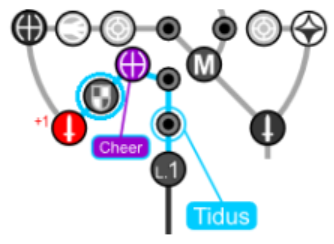
\includegraphics[width=.7\columnwidth]{graphics/tiduscheer}}{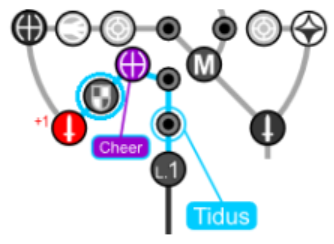
\includegraphics[width=.4\columnwidth]{graphics/tiduscheer}}
    \end{itemize}
\end{spheregrid}
\begin{battle}[750]{Kimahri}
    Each Attack does average of 125, count damage compared to average to know if you need to Potion or not.
    If you did the above sphere grid already, 6 Attacks will always kill.
    \begin{itemize}
        \tidusf Attack x5
        \item \textit{If the Attacks did at least 7 damage over average:}
        \begin{itemize}
            \tidusf Attack
        \end{itemize}
        \item \textit{If \tidus\ has less than 178 HP:}
        \begin{itemize}
            \tidusf Potion
        \end{itemize}
        \tidusf Attack x1-2
    \end{itemize}
\end{battle}
\begin{enumerate}[resume]
    \item \sd, continue running
\end{enumerate}
\begin{battle}{Garuda}
    \begin{itemize}
        \summon{\valefor}
        \valeforf Thunder x6 to build \od
    \end{itemize}
    Guaranteed 1 Power Sphere.
\end{battle}
\begin{enumerate}[resume]
    \item If you didn't do the above sphere grid yet, do it now (only get Cheer if Tidus has 2 levels).
    \item \formation{\tidus}{\yuna}{\lulu}
\end{enumerate}
\begin{battle}{Garuda}
    \begin{itemize}
        \item Flee using the Escape Command
    \end{itemize}
\end{battle}
\begin{encounters}
    \begin{itemize}
        \item Dingo: \tidus\ Attack
        \item Condor: \wakka\ Attack
        \item Water Flan: \lulu\ Thunder
    \end{itemize}
\end{encounters}
\begin{enumerate}[resume]
    \item At Besaid Beach \save, talk to the guy in red shorts for 400 Gil, go onto the boat.
\end{enumerate}
    \chapter{S.S. Liki}

\begin{enumerate}
    \item \cs[2:00], walk up to \yuna, \sd, walk back to \wakka, \sd, walk back up to \yuna, \cs + 4 \skippablefmv[4:20], \sd\ from `Sin!'
\end{enumerate}
\begin{battle}[2000]{Sin Fin}
    \begin{itemize}
        \tidusf Defend
        \switch{\yuna}{\lulu}
        \luluf Thunder the Sin Fin
        \switch{\kimahri}{\yuna}
        \summon{\valefor}
        \valeforf Energy Ray \od\ on Sin Fin
        \enemyf Move x2 and Spines x2
        \valeforf Thunder the Sin Fin
        \enemyf Spines and Move
        \valeforf Thunder the Sin Fin x2
        \item \textit{If Sin Fin is not dead yet:}
        \begin{itemize}
            \enemyf Spines
            \switch{\tidus}{\wakka}
            \wakkaf Attack the Sin Fin
        \end{itemize}
    \end{itemize}
\end{battle}
\begin{enumerate}[resume]
    \item \fmv+\cs[1:40]
\end{enumerate}
\begin{battle}[2000]{Sinspawn Echuilles}
    \begin{itemize}
        \tidusf Cheer x2
        \wakkaf Dark Attack
        \tidusf Attack x2 \textit{if Str Node else} Cheer x2
        \wakkaf Attack x2
        \enemyf Blender
        \wakkaf Attack x2
        \tidusf Attack x2, one less if either \tidus\ crits or \wakka\ crits twice.
        \tidusf \od
    \end{itemize}
    Check for \textbf{Ice Brand, Ice Ball}
\end{battle}
\begin{enumerate}[resume]
    \item \skippablefmv+\cs[1:30], \sd\ during \tidus\ monologue.
\end{enumerate}
    \chapter{Kilika}

\begin{enumerate}
    \item \sd\ on exiting the boat, go up and left, \sd. \skippablefmv[2:00], (press Start immediately after skip) \sd
    \item Exit inn, go right to \wakka, \sd. Go left and up to Kilika Woods, \sd
\end{enumerate}
\begin{battle}{Lancet Tutorial}
    \begin{itemize}
        \item \sd
        \kimahrif Lancet
        \switch{\kimahri}{\wakka}
        \wakkaf Defend
        \tidusf Attack
        \item \textit{If Valefor died on Sin Fin:}
        \begin{itemize}
            \switch{\lulu}{\yuna}
            \summon{\valefor}
            \valeforf Boost x2
            \valeforf Fire
        \end{itemize}
        \item \textit{Else:}
        \begin{itemize}
            \luluf Fire
        \end{itemize}
    \end{itemize}
\end{battle}
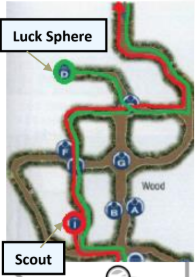
\includegraphics{graphics/kilikamap}
\begin{enumerate}[resume]
    \item Go left and up the hidden path, \pickup{Scout}
\end{enumerate}
\begin{spheregrid}
    \begin{itemize}
        \tidusf
        \begin{itemize}
            \item Move $\leftarrow\leftarrow$ or $\nwarrow$
            \item Flee, Agi+1 (, Str +1 if you didn't get it already)
        \end{itemize}
        \sggraphics{.7}{.4}{graphics/Tidus_Kilika}
    \end{itemize}
\end{spheregrid}
\begin{equip}
    \begin{itemize}
        \wakkaf Scout/Ice Ball
        \wakkaf Any Armguard (optional)
        \tidusf Ice Brand (optional)
    \end{itemize}
\end{equip}
\begin{enumerate}[resume]
    \item \formation{\tidus}{\wakka}{\lulu}
    \item Continue up the hidden path, following the map. Fight encounters as described below.
    \item Need 45 AP on \tidus, which is 5 kills (Overkills count as 2). This is your main source of Speed Spheres but you can obtain the rest later.
    \item You can benefit from kills beyond the first 5 but do not intentionally farm encounters and stop killing if you have 17 kills already.
\end{enumerate}
\begin{encounters}
    \begin{itemize}
        \item \textit{If there is only Ragoras:}
        \begin{itemize}
            \tidusf Flee
        \end{itemize}
        \tidusf Attack the Dinonix if present, else Defend
        \wakkaf Attack the Killer Bee if present, else Defend
        \luluf Water the Yellow Element or Killer Bee
        \tidusf Flee
    \end{itemize}
\end{encounters}
\begin{enumerate}[resume]
    \item \sd
    \item \formation{\tidus}{\yuna}{\lulu}
    \item \save
\end{enumerate}
\begin{battle}[3000]{Sinspawn Geneaux}
    \begin{itemize}
        \item \textit{If \tidus\ is going before \yuna:}
        \begin{itemize}
            \tidusf Defend
        \end{itemize}
        \item \textit{Else:}
        \begin{itemize}
            \switch{\yuna}{\wakka}
            \wakkaf Defend
            \tidusf Defend
            \switch{\lulu}{\yuna}
        \end{itemize}
        \summon{\valefor}
        \valeforf \od\ Energy Ray
        \valeforf Fire x3
        \valeforf \od\ Energy Ray
    \end{itemize}
    Guaranteed 4 Power Spheres, if Rare Drop from Geneaux +2 Power Spheres.
\end{battle}
\begin{enumerate}[resume]
    \item \sd\ on stone steps and temple. go into temple. Walk up to \wakka\ and Pray. \sd\ inside temple and go up steps. Wait for lift and \sd.
\end{enumerate}
\begin{trial}
    \begin{itemize}
        \item Take the sphere from the pedestal
        \item Place into the door, take it off of the door.
        \item Place sphere into the next door, take the sphere back.
        \item Place the sphere into the right holder
        \item Touch glpyh
        \item Take the sphere from the next room
        \item Place it into the left holder
        \item Take the glyph sphere from the pedestal
        \item Place it in the Fire Room
        \item Take the sphere that you put into the right holder
        \item Use it to open the door in the Fire Room
        \item Take the sphere off the door
        \item Enter the Fayth room
    \end{itemize}
\end{trial}
\begin{enumerate}[resume]
    \item In Fayth room, \sd, speak to \wakka\ first. Try to leave room, \sd, name \ifrit
    \item Hold down to exit temple, \cs[0:40], \sd
    \item \formation{\tidus}{\wakka}{\lulu}
    \item Go south through Kilika Woods, take the left path and \pickup{Luck Sphere}, referencing the above map.
    \item Exit Kilika Woods same way that you entered, treating fights the same way as above.
    \item Do the below Sphere Grid if \tidus\ has 5 S.Levels.
    \item Go down and right to S.S. Winno. \sd
\end{enumerate}

    \chapter{S.S. Winno}
\begin{enumerate}
    \item \cs[1:10], exit door on the right. \sd\ with Oaka. Run outside, go up to the top deck for \wakka\ and \lulu\ cutscene, \sd
    \item Run up the blitzball on the front of the boat. \cs[1:10]
    \item Follow the tutorial, fail the minigame. Do \textbf{not} get Jecht Shot.
    \item \sd\ on \yuna's scene, do not save. \skippablefmv[0:30] if you buffered the Start command in Kilika.
\end{enumerate}
    \chapter{Luca}

\begin{enumerate}
    \item \sd, go right and up to the next screen, \cs[2:30]. Don't save.
    \item \sd\ in locker room. Don't do the tutorial. \sd\ by mashing another button (like \textbf{R1}) at the same time as confirm, walk down, \sd
    \item Walk down to next screen, \sd. Whistle \cs[0:30], walk right to next screen.
    \item \sd, run to the cafe. \sd, \skippablefmv+\cs[1:20], \sd
    \item Run left to next screen, then left to the docks.
    \item Talk to O'aka on the first docks screen, before going into the Machina Fights. Do the following shop:
    \begin{shop}{3050}
        \begin{itemize}
            \item Sell
                  \begin{itemize}
                      \item All Weapons and Armor other than Official Ball, Lightning Steel, Thunder Ball.
                  \end{itemize}
            \item Buy
                  \begin{itemize}
                      \item Stunning Steel, Equip
                  \end{itemize}
            \item If you don't have enough gil after selling Equipment, on the same dock as O'aka there are 2 chests with 600 Gil and a Tidal Spear you can sell
        \end{itemize}
    \end{shop}
    \item Run north to the next screen.
\end{enumerate}
\begin{battle}{Machina - First Two Encounters}
        \begin{itemize}
            \item \textit{No Early Haste}
            \begin{itemize}
                \tidusf Defend
                \kimahrif Defend
                \luluf Thunder
            \end{itemize}
            \item \textit{Early Haste}
            \begin{itemize}
                \tidusf Haste Lulu, then Defend
                \kimahrif Defend
                \luluf Thunder
            \end{itemize}
        \end{itemize}
\end{battle}
\begin{enumerate}[resume]
    \item Do the below Sphere Grid if \tidus\ has 5 S.Levels.
\end{enumerate}
\vfill
\begin{battle}{Machina Third Encounter}
        \begin{itemize}
        \item \textit{No Early Haste}
        \begin{itemize}
            \item \textit{First Wave}
            \begin{itemize}
                \tidusf Attack
                \kimahrif Attack
                \luluf Thunder a different Machina
                \tidusf Attack
                \kimahrif \od\ Seed Cannon \textit{if no crits else} Attack
            \end{itemize}
            \item \textit{Second Wave}
            \begin{itemize}
                \tidusf Defend
                \kimahrif Defend
                \luluf Thunder
            \end{itemize}
            \item \textit{Third Wave}
            \begin{itemize}
                \tidusf Attack
                \kimahrif Attack or \od\ Seed Canon
                \luluf Thunder a different Machina
            \end{itemize}
        \end{itemize}
        \item \textit{Early Haste}
        \begin{itemize}
        \tidusf Haste Lulu, then Defend
        \kimahrif Defend
        \luluf Thunder
        \end{itemize}
    \end{itemize}
\end{battle}
\begin{enumerate}[resume]
    \item If anyone is Critical HP, use Potions. If you had Early Haste, take the Save Sphere to restore \tidus's MP.
    \item Do the below Sphere Grid if \tidus\ has 5 S.Levels.
    \item Run right.
\end{enumerate}
\begin{battle}[3000]{Oblitzerator}
    \begin{itemize}
        \kimahrif Defend
        \tidusf Defend \textit{If No Early Haste Else} Haste \lulu
        \luluf Thunder Crane x3
        \tidusf Use Crane after \lulu's 3rd Thunder
        \kimahrif Defend
        \luluf Thunder
        \tidusf Attack
    \end{itemize}
    Check for \textbf{Lightning Steel, Thunder Ball}
\end{battle}
\begin{enumerate}[resume]
    \item \cs[2:00], \sd\ during and after Blitzball game.
\end{enumerate}
\begin{spheregrid}
    \begin{itemize}
        \tidusf (5 S.Lvl)
        \begin{itemize}
            \item Move $\downarrow \searrow\searrow$
            \item +1 Str, Haste, +20 MP
        \end{itemize}
    \end{itemize}
    \ifthenelse{\equal{\colstyle}{multi}}{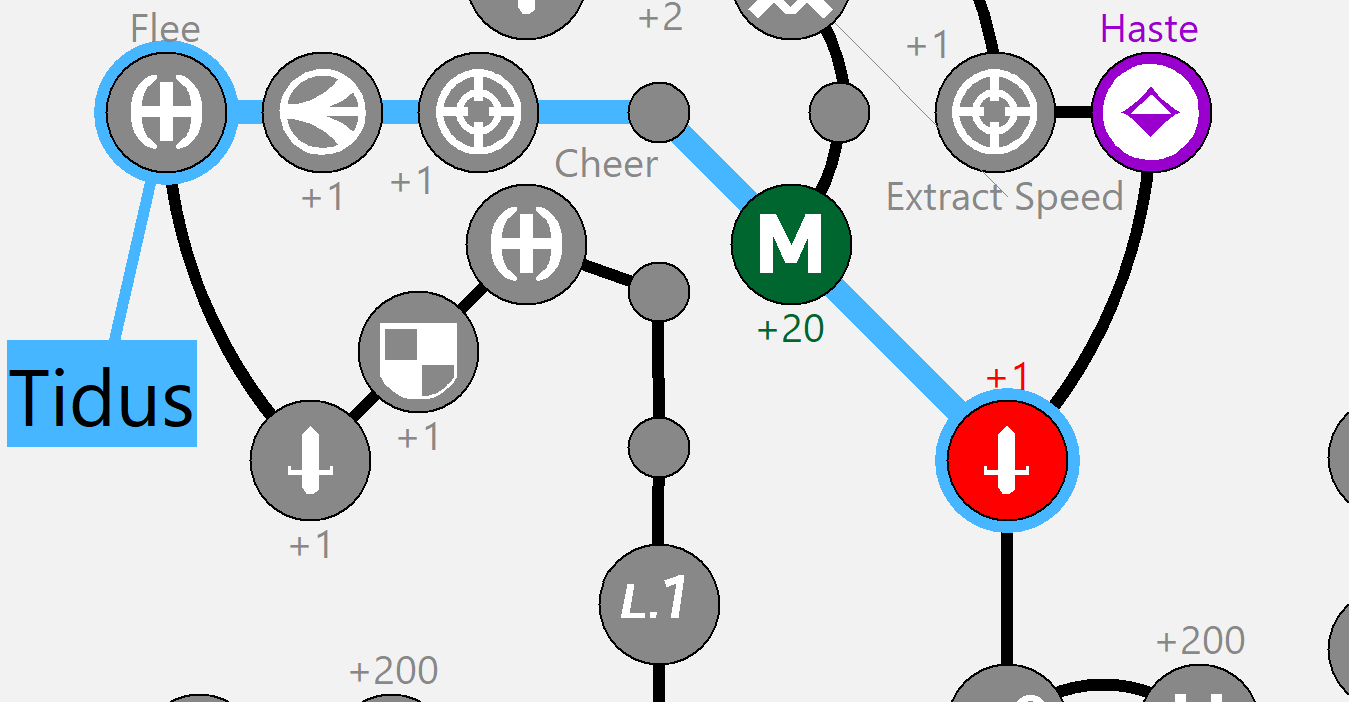
\includegraphics[width=.6\columnwidth]{graphics/haste}}{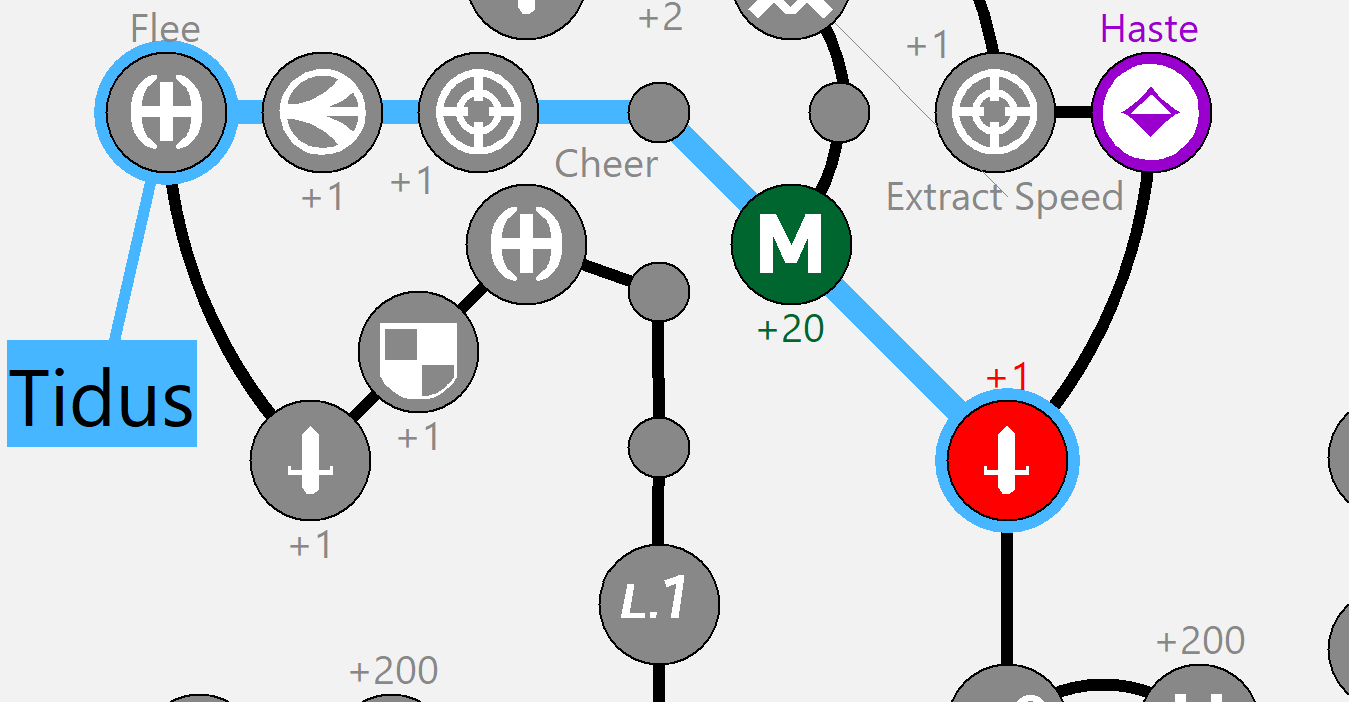
\includegraphics[width=.3\columnwidth]{graphics/haste}}
\end{spheregrid}
\begin{equip}
    \begin{itemize}
        \item \textit{If you got Thunder Ball}
        \begin{itemize}
            \wakkaf Thunder Ball
            \item \textit{If you also got Lightning Steel}
            \begin{itemize}
                \tidusf Lightning Steel
            \end{itemize}
        \end{itemize}
    \end{itemize}
\end{equip}
\begin{enumerate}[resume]
    \item Run South for the next two screens. \save. Go up the stairs to the locker room, \sd
    \item Go back into locker room, speak to \wakka, \sd, \cs[1:20]. \sd\ after \lulu\ scene. \cs[1:40] on \auron\ Entrance.
\end{enumerate}
\bothvfill\winvfill\lossvfill
\begin{blitzball}
    \begin{itemize}
        \item \textbf{First Half:}
        \begin{itemize}
            \item \textit{If Luca wins the Blitzoff:}
            \begin{itemize}
                \item Triangle, switch the mode to \textbf{Mark Mode}, and then \textbf{Left Side}
            \end{itemize}
            \item \textit{When you get the ball:}
            \begin{itemize}
                \item Change to \textbf{Manual A} and \textbf{Normal Mode}
                \item down some, pass the ball to \tidus
                \tidusf Swim next to Jassu, pass to Jassu
                \item Hide behind the Goalie
                \item If you aggroed a Goer, Swim Around
            \end{itemize}
        \end{itemize}
        \item \sd\ during half time
        \item \textbf{Second Half:}
        \begin{itemize}
            \item \textit{If Luca wins the Blitzoff:}
            \begin{itemize}
                \item Triangle, switch the mode to \textbf{Mark Mode}, and then \textbf{Right Side}
            \end{itemize}
            \item \textit{When you get the ball:}
            \begin{itemize}
                \item Pass to Jassu if he doesn't have it
                \item Swim to the Bottom Middle
                \item Wait until 2:20, if Abus Aggros then Break
                \item Swim to the Left, aggro Balgerda (bottom player), then swim back some
                \item Pass to \tidus\ before Balgerda gets in range to block
                \tidusf Swim close to the Goal and Sphere Shot before anyone is close enough to block
                \begin{itemize}
                    \item If 1 Defender and 2:49, Sphere Shot over the Defender
                    \item Otherwise, Break and Sphere Shot
                    \item If 2 Defenders, Break 1, Sphere Shot
                \end{itemize}
            \end{itemize}
            \item \sd\ during \wakka\ \cs
            \item If you need to Score or it's 1-1, then do the same as above with Jassu
            \item Wait until 4:20 then aggro Balgerda, Pass to \wakka
            \wakkaf swim close and Venom Shot, or Break, Venom Shot
        \end{itemize}
        \item Don't try to score in the First Half
        \item If you're losing, Change to \textbf{Mark Mode} and lose the game.
    \end{itemize}
\end{blitzball}
\begin{enumerate}[resume]
    \item \sd, Don't Save, \cs[1:00]
\end{enumerate}
\bothvfill\winvfill\lossvfill
\begin{battle}{Sahagin Chief}
    \begin{itemize}
        \item \textit{If no Thunder Ball:}
        \begin{itemize}
            \tidusf Haste \tidus
            \wakkaf For the first two waves Attack Sahagin C
            \wakkaf For the third wave Potion \tidus\ if he has less than 156 HP, otherwise Defend
        \end{itemize}
        \item \textit{If Thunder Ball:}
        \begin{itemize}
            \tidusf Cheer
            \wakkaf Attack
            \tidusf Haste \tidus
            \tidusf Haste \wakka
            \item \textit{If also Lightning Steel:}
            \begin{itemize}
                \tidusf Cheer
            \end{itemize}
        \end{itemize}
        \tidusf Attack
    \end{itemize}
    Guaranteed 17 Power Spheres. Each Overkill is +1 Power Sphere
\end{battle}
\begin{enumerate}[resume]
    \item \sd, \skippablefmv. Overkill on Vouivre is +1 Power Sphere
\end{enumerate}
\begin{battle}[1800]{Garuda}
    \begin{itemize}
        \tidusf Haste \auron
        \auronf Attack x3
        \wakkaf Defend, Potion if \tidus\ has less than 312 HP
        \tidusf Attack x1, then Defend
        \wakkaf Defend, Potion if \auron\ has less than 202 HP
        \auronf Attack x3
        \item Don't revive non-\auron\ party members
    \end{itemize}
    Guaranteed 2 Power Spheres from this and the Vouivre. Overkill is +1 Power Sphere
\end{battle}
\begin{enumerate}[resume]
    \item \cs+\skippablefmv[1:30], buffer the FMV Skip. Don't save. \sd\ the Auroch scene
    \item \cs[4:50]. Run north to the hidden chests, \pickup{Magic and HP Sphere}
    \item Run South and try to speak to \auron\ while he's walking away.
    \item Follow red arrow to \yuna. \sd\ during guardian scene. Walk to \yuna, \cs[4:20]
\end{enumerate}
    \chapter{Mi'ihen Highroad}

\begin{enumerate}
	\item Walk up. Forced encounter, \sd. Walk up, \sd\ during Maechen Scene. Guaranteed 1 Power Sphere from the tutorial, +1 if Overkill.
	\item \formation{\tidus}{\wakka}{\auron}
	\item Flee from every encounter
	\item Heal using \yuna's Cure if \tidus\ is in crit and after every Ambush
\end{enumerate}
\bothcb\wincb\losscb
\begin{enumerate}[resume]
	\item {Mi'ihen Skip}
		\begin{itemize}
			\item After Maechen Scene, run up as quickly as possible.
			\item Go to the White Spot on the ground towards the left before the Man in Blue
			\item Speak to the man, get the \textbf{Hunter's Spear}
			\item Mash and step forward over the cutscene line
			\item Walk up during the cutscene after the teleport to the next screen.
		\end{itemize}
	\item Make sure you get the \textbf{Hunter's Spear} if you fail the skip.
	\item Go right and \sd\ at Calli scene. Continue walking up. \sd\ Luzzu scene, \sd\ Shelinda scene
	\item Go to the next screen
	\item Go to the Al-Bhed shop, \sd. Walk out of the shop and \cs[5:30]
	\item Leave shop, \sd. \sd\ on Rin. Walk outside.
\end{enumerate}
\begin{battle}{Chocobo Eater}
	\begin{itemize}
		\tidusf Haste Boss
		\item Defend with everyone.
		\item Swap any characters that fall into crit HP with someone in the back.
	\end{itemize}
\end{battle}
\begin{enumerate}[resume]
	\item \sd
	\item \formation{\tidus}{\wakka}{\auron}
	\item Walk north, \save. Walk north to next screen. Walk to blocked road, \sd. Speak to the guard on the right, \sd, walk back, \sd. Walk up to next screen.
\end{enumerate}
    \chapter{Mushroom Rock Road}

\begin{enumerate}
	\item \sd, \cs.
	\item Clasko Skip
	      \begin{itemize}
		      \item Run forward to the 3 Soldiers
		      \item Wedge yourself behind the right soldier by holding Left for a second
		      \item Tap Down-Right, X to speak to the bottom soldier
		      \item If the Soldier got away:
		            \begin{itemize}
			            \item Run up near the white spot on the wall near the trigger
			            \item Talk to the Soldier right after he pushes you into the trigger
			            \item Mash until trigger dialogue during the \cs
		            \end{itemize}
	      \end{itemize}
	\item Flee from any encounters, go to the next screen.
	\item \save. Go back to the previous screen
	\item Perform MRR Skip. For a tutorial, please see \href{https://www.youtube.com/watch?v=SSnxE6Xzvkk}{this tutorial}.
	\item \sd\ during \tidus\ monologue. \cs[1:00], \sd
	\item Walk left, \save, \sd. Walk left, speak to \auron, \sd. Go up and right, \sd, exit area, \sd.
\end{enumerate}
\bothvfill\winvfill\lossvfill
\ 
\bothcb\wincb\losscb

    \chapter{Djose}
\begin{enumerate}
    \item Walk North, if by the end of the road you have not found a Basilisk, force more encounters until you get one, now or after you exit Djose Temple.
\end{enumerate}
\begin{encounters}
    \begin{itemize}
        \item Basilisk:
        \begin{itemize}
            \switch{anyone}{\kimahri}
            \kimahrif Lancet Basilisk, learn \textbf{Stone Breath}
            \item Flee.
        \end{itemize}
        \item Else Flee
    \end{itemize}
\end{encounters}
\begin{enumerate}[resume]
    \item Continue walking north, \sd, walk up to the next screen.
    \item Walk along bridge to next screen, \sd, walk into temple. Speak to \auron\ at the doorway, \sd, walk up the stairs.
\end{enumerate}
\bothvfill\winvfill\lossvfill
\begin{trial}
    \begin{itemize}
        \item Take the sphere from the left wall
        \item Place into door
        \item Take the sphere from the right wall
        \item Place into door
        \item Take the sphere from the left wall
        \item Push pedestal to the right
        \item Put sphere into the far right wall
        \item Take right sphere
        \item Place into the far right wall
        \item \cs
        \item Take sphere from far right wall
        \item Reset puzzle with the far left tile
        \item Place sphere into pedestal
        \item Take the pedestal sphere
        \item Put sphere into right wall
        \item Take the far right sphere
        \item Put into pedestal
        \item Push pedestal through the door
        \item Jump onto pedestal
        \item Push the second pedestal, return to main room
        \item Take the charged sphere from the right wall
        \item Place charged sphere into the left wall
        \item Reset
        \item Place the two pedestal spheres in the first left and right walls
        \item Go onto the lift in the center
        \item Push all the pedestals in, walk up the stairs
    \end{itemize}
\end{trial}
\begin{enumerate}[resume]
    \item Talk to \auron, wait. \sd, try to leave, \sd, name \ixion
    \item Speak to \auron, enter the temple and go to the left room. Speak to the priest, \sd. Exit the temple, \sd
    \item Go left, \pickup{4000 Gil}, cross the bridge, \sd, exit, \sd, go up to Moonflow.
\end{enumerate}
    \chapter{Moonflow}

\begin{enumerate}
	\item Walk north, \sd\ on \kimahri\ Scene.
	\item Before Belgemine, go right into alcove and \pickup{Lv. 1 Key Spheres x3}
	\item Walk north, \sd, walk left, \sd, walk left past 2 screens, \sd.
\end{enumerate}
\begin{spheregrid}
	\wakkaf (7 S.Lvl)(if you don't have enough, skip this Grid entirely)
	\begin{itemize}
		\item Move $\rightarrow x4 (\downarrow)$Silence Attack
		\item +2 Strength
	\end{itemize}
	\ifthenelse{\equal{\colstyle}{multi}}{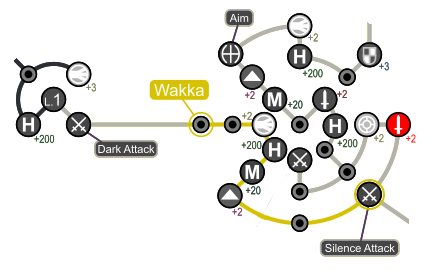
\includegraphics[width=.9\columnwidth]{graphics/Wakka_Grid}}{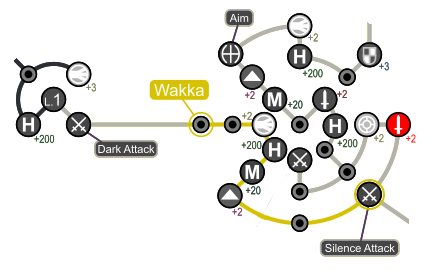
\includegraphics[width=.45\columnwidth]{graphics/Wakka_Grid}}
\end{spheregrid}
\begin{enumerate}[resume]
	\item Potion/Cure \tidus\ if he got injured. Walk right and use the \nth{2} option to ride ze shoopuf, \sd.
\end{enumerate}
\bothvfill\winvfill\lossvfill
\begin{battle}[4000]{Extractor}
	\begin{itemize}
		\tidusf Haste self
		\wakkaf Attack
		\tidusf Attack Extractor until you apply Slow
		\item \textit{If Extractor is not Slowed when it Rises:}
			\begin{itemize}
				\wakkaf \od\ Thunder Reels.
			\end{itemize}
		\tidusf Haste Wakka
		\tidusf \textit{If Lightning Steel:}
			\begin{itemize}
				\tidusf Cheer x1
				\tidusf Equip Lightning Steel
			\end{itemize}
		\textit{Else:}
			\begin{itemize}
				\tidusf Cheer x1
				\tidusf Equip Brotherhood
			\end{itemize}
		\tidusf Attack
	\end{itemize}
\end{battle}
\begin{enumerate}[resume]
	\item \sd, walk left to next screen, walk left and talk to \rikku, \sd
	\item Walk up to the forced encounter
\end{enumerate}
\begin{battle}{Rikku Tutorial}
	\begin{itemize}
		\item Mash through the tutorial
		\rikkuf Steal from the Treasure Chest
		\item \textit{If you have less than 34 Power Spheres:}
		      \begin{itemize}
			      \rikkuf \od\ Two Ability Spheres
		      \end{itemize}
		\item \textit{Else:}
		      \begin{itemize}
			      \rikkuf \od\ Two Potions
				  \rikkuf Defend
				  \item Flee
		      \end{itemize}
	\end{itemize}
+2 Power Spheres when doing the Ability Sphere Mix.
\end{battle}
\begin{spheregrid}
	\begin{itemize}
		\tidusf (4 S.Lvl)
		\begin{itemize}
			\item Move $\rightarrow\uparrow$
			\item Str+1, HP+200, Agil+2
		\end{itemize}
		\ifthenelse{\equal{\colstyle}{multi}}{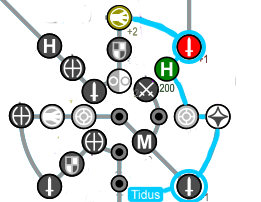
\includegraphics[width=.6\columnwidth]{graphics/Tidus_post_gui}}{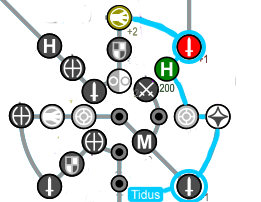
\includegraphics[width=.35\columnwidth]{graphics/Tidus_post_gui}}
	\end{itemize}
\end{spheregrid}
\begin{enumerate}[resume]
	\item Auto-Sort items
	\item Heal everyone with Potions (use them all if you can to free up the 1st Inventory Slot)
	\item If your 1st Inventory Slot is not empty Manual sort the item in that slot 1 page down
	\item \formation{\tidus}{\wakka}{\auron}
	\item Walk north to next screen.
\end{enumerate}
    \chapter{Guadosalam}

\begin{enumerate}
	\item \sd, walk to Seymour's house, try to leave. Walk into room, speak to \auron, \sd, speak to \wakka, \lulu, \rikku, \yuna. \sd, \skippablefmv+\cs[5:50] if you buffered the Start command after Gui.
	\item Exit the house, walk down, \sd. Go to the Farplane. Hidden to the left in the screen going to the Farplane, \pickup{Lightning Marble x8}
	\item \sd, speak to \auron, go into the Farplane. \cs[1:20]. Speak to \wakka, \sd, speak to \yuna, \cs[2:10], \sd.
	\item Go to Seymour House Entrance, \sd
	\bothcb \wincb \losscb
	\item Guadosalam Skip:
	      \begin{itemize}
		      \item Stand outside of the Potion Shop
		      \item Wait until you get pushed by the Guado to trigger the skip
		      \item Run to the exit using the minimap
		      \item If on HD Remaster, speak to the woman on the left to stop her walking abit, then speak to the running Guado as the woman pushes you to into the door.
	      \end{itemize}
	      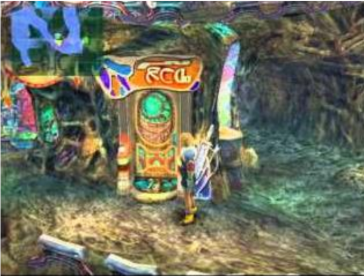
\includegraphics{graphics/guadoskipstandard}

	      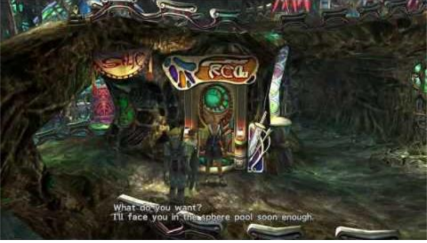
\includegraphics{graphics/guadoskipremaster}
\end{enumerate}
    \chapter{Thunder Plains}

\begin{enumerate}
    \item Walk north, dodging lightning, Flee all encounters.
\end{enumerate}
\begin{enumerate}[resume]
    \item \sd\ when approaching Al Bhed shop. Walk into the shop when \rikku\ begs to go inside.
\end{enumerate}
\begin{shop}{1200+}
    \begin{itemize}
        \blitzballdetermination[true]{%
            \item Items menu only.
        }{%
            \item Sell: 1st Equipment on the 2nd page (after the equipped ones)
            \item Sell: Other Equipment worth 1k+ Gil
            \item Buy: Baroque Sword (Equip)
        }
        \item Buy:
        \begin{itemize}
            \item 3 Phoenix Downs
            \ifthenelse{\equal{\blitzresult}{win}}{%
                \item 3 Grenades
            }{\ifthenelse{\equal{\blitzresult}{both}}{%
                \item 3 Grenades, +1 if \blitzloss
            }{%
                \item 4 Grenades
            }}, +1 for every 3 Speed Spheres you are missing (need 15 Speed Spheres for the rest of the run)
        \end{itemize}
    \end{itemize}
    Try to leave the shop with at least 6839 Gil.
\end{shop}
\begin{enumerate}[resume]
    \item Walk into shop corridor, \cs[2:00]
    \item Speak to \auron, then to \rikku, \sd.
    \item Pickup the \textbf{Yellow Shield} outside the shop on the ground.
    \item Try to end Thunder Plains with the Light Curtain.
\end{enumerate}
\begin{equip}
\begin{itemize}
\tidusf Yellow Shield
\end{itemize}
\end{equip}
\begin{encounters}
    Iron Giants will always target the Character with the least HP, make sure everyone's HP is above Rikku's
    \begin{itemize}
        \item Iron Giant + 2 Buers, if you bought extra Grenades for Speed Spheres:
        \begin{itemize}
            \switch{\tidus}{\rikku}
            \rikkuf Use Grenade
            \wakkaf Defend
            \auronf Defend
            \enemyf Attacks \rikku
            \switch{\wakka}{\tidus}
            \item Flee
        \end{itemize}
        \item Iron Giant:
        \begin{itemize}
            \tidusf Defend
            \switch{\wakka}{\rikku}
            \rikkuf Steal Light Curtain
            \auronf Defend
            \enemyf Attacks \rikku
            \item Flee
        \end{itemize}
        \blitzballdetermination[true]{}{\item Larva: Steal Lunar Curtain}
    \end{itemize}
\end{encounters}
\begin{enumerate}[resume]
    \item Exit screen, go north, near the exit \sd, \cs[3:10]
\end{enumerate}
    \chapter{Macalania Woods}

\begin{enumerate}
	\item \sd, walk north, \sd, \save
	\item \formation{\tidus}{\rikku}{\auron}
	\item Follow path, \pickup{2000 Gil}
	\item Cure \tidus\ if he's ever below 404 HP.
	\item Make sure that you charge \rikku\ \od, and that you do at least one of each of the following steals.
\end{enumerate}
\begin{encounters}
	\begin{itemize}
		\item Chimera: Steal Arctic Wind, Flee
		\item Blue Elemental: Steal Fish Scale x2, Flee
		\item Else: Flee
	\end{itemize}
\end{encounters}
\begin{enumerate}[resume]
	\item Once \rikku\ has \od\ and you have at least 1 Arctic Wind and 1 Fish Scale, \formation{\tidus}{\yuna}{\kimahri}
	\item Follow path, \sd\ twice
	\item Catch butterfly near the exit to avoid encounters
	\formation{\tidus}{\yuna}{\kimahri}
	\item \save, talk to O'aka, pick the first option ("Got any weapons?"), exit the shop, pick the first option ("Too pricey."), talk to him again ("Got any weapons?")
\end{enumerate}
\begin{shop}{11550}
	\begin{itemize}
		\item Sell: Stunning Steel, Buckler, Hunter Spear, any other equipment to go above 11550 Gil
		\item Buy:
			\begin{itemize}
				\item Sonic Steel, Equip
				\item Shimmering Blade, Equip
			\end{itemize}
	\end{itemize}
\end{shop}
\begin{enumerate}[resume]
	\item Run up, \sd. Enter the hidden path, walk to \auron, \sd
\end{enumerate}
\bothvfill\winvfill\lossvfill
\begin{battle}[12000]{Spherimorph}
	\begin{itemize}
		\tidusf Change Weapon to Sonic Steel
		\tidusf Defend
		\switch{\tidus}{\rikku}
		\rikkuf Grenade, check the Element
		\item \kimahri\ and \yuna: If anyone is dead \textbf{Phoenix Down}, otherwise Defend
		\rikkuf \od, HP Sphere with
		\begin{itemize}
			\item Fire: Arctic Wind
			\item Ice: Bomb Core
			\item Water: Lightning Marble
			\item Thunder: Fish Scale
		\end{itemize}
		\item \textit{If you don't have the elemental item:}
			\begin{itemize}
				\switch{\rikku}{\lulu}
				\luluf Use the spell opposite of what Spherimorph used
				\yunaf Defend
				\kimahrif Attack, check the Element
				\switch{\lulu}{\rikku}
				\rikkuf \od
			\end{itemize}
	\end{itemize}
	\tidus, \yuna, \kimahri, \rikku\ all need AP.
\end{battle}
\begin{enumerate}[resume]
	\item \cs[1:50], \sd, \sd
\end{enumerate}
\colend
\begin{spheregrid}
	\begin{multicols}{2}
		\begin{itemize}
			\rikkuf (1 S.Lvl)
			\begin{itemize}
				\item Move $\downarrow$
				\item Agi+3
			\end{itemize}
			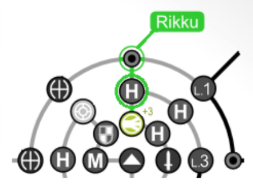
\includegraphics[width=.5\columnwidth]{graphics/macalaniarikku}
			\kimahrif (15 S.Lvl)
			\begin{itemize}
				\item Move $\downarrow x7$ or $\swarrow\swarrow\downarrow\downarrow$, next to Lv. 1 Lock
				\item Level 1 Key Sphere
				\item Move $\leftarrow\leftarrow\leftarrow\leftarrow$
				\item Level 1 Key Sphere
				\item Move $\uparrow\uparrow\leftarrow$
				\item Steal, Use
			\end{itemize}
			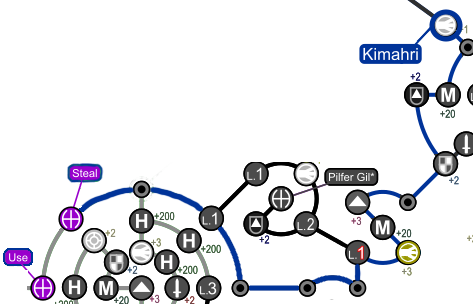
\includegraphics[width=.8\columnwidth]{graphics/Kimahri_post_spheremorph}
		\end{itemize}
	\end{multicols}
\end{spheregrid}
\colstart
\begin{enumerate}
	\setcounter{enumi}{10}
	\item \formation{\tidus}{\lulu}{\kimahri}
	\ifthenelse{\equal{\blitzresult}{both}}{%
		\item If \blitzloss\ and don't have a Light Curtain heal everyone
	}{\ifthenelse{\equal{\blitzresult}{loss}}{%
		\item If you don't have a Light Curtain heal everyone
	}{}}
	\item Talk to \auron\ on the way out, then exit
\end{enumerate}
\newpage
    \chapter{Lake Macalania}

\begin{enumerate}
    \item Run up and \sd
\end{enumerate}
\begin{battle}[16000]{Crawler}
    \begin{itemize}
        \switch{\tidus}{\rikku}
        \rikkuf Lightning Marble x1/2 Negator (1\,000 HP)
        \rikkuf Lightning Marble Crawler
        \kimahrif Lightning Marble Crawler
        \luluf Phoenix Down \rikku
        \rikkuf Lightning Marble Crawler
        \ifthenelse{\equal{\blitzresult}{win}}{%
            \switch{\lulu}{\yuna}
            \yunaf Mega Phoenix
            \switch{\yuna}{\tidus}
            \tidusf Equip Brotherhood
        }{\ifthenelse{\equal{\blitzresult}{loss}}{%
            \kimahrif If you need a Lunar Curtain Steal Crawler, else Defend
            \switch{\lulu}{\yuna}
            \yunaf If 2 Characters dead Mega Phoenix, else Phoenix Down \rikku
            \switch{\yuna}{\tidus}
            \tidusf If \kimahri\ is dead Phoenix Down him, otherwise Equip Brotherhood
        }{%
            \kimahrif If \blitzloss\ and you need a Lunar Curtain Steal Crawler, else Defend
            \switch{\lulu}{\yuna}
            \yunaf If 2 Characters dead Mega Phoenix, else Phoenix Down \rikku
            \switch{\yuna}{\tidus}
            \tidusf If \kimahri\ is dead Phoenix Down him, otherwise Equip Brotherhood
        }}
        \rikkuf \od\ Lv. 2 Key Sphere and Lightning Marble
    \end{itemize}
    \tidus, \yuna, \lulu\ and \kimahri\ need AP.
\end{battle}
\bothvfill
\winvfill
\lossvfill
\begin{spheregrid}
    \begin{itemize}
        \kimahrif (12 S.Lvl)
        \begin{itemize}
            \item Move $\downarrow\downarrow\downarrow\downarrow$ on the Luck node
            \item HP +200, Agi+4
        \end{itemize}
        \sggraphics{.7}{.4}{graphics/macalania_kimahri}
        \tidusf (22 S.Lvl)
        \begin{itemize}
            \item Level 2 Key Sphere
            \item Move $\rightarrow\uparrow$
            \item Str +4
            \item Move $\uparrow\uparrow$
            \item HP+200
            \item Move $\rightarrow\rightarrow\uparrow$
            \item HP+200, Str+4, Agi+2
            \blitzballdetermination[true]{%
                \item Move $\rightarrow$
                \item Use Strength Sphere, Activate it
                \item Move $\uparrow\leftarrow\leftarrow$ or $\nwarrow\nwarrow$
            }{%
                \item Move $\uparrow\leftarrow$
            }
            \item HP+200, Str+4, Agi+2
            \item Move $\leftarrow$
            \item Str+4
        \end{itemize}
        \ifthenelse{\equal{\blitzresult}{win}}{%
            \sggraphics{.7}{.4}{graphics/Tidus_post_crawler}
        }{\ifthenelse{\equal{\blitzresult}{both}}{%
            \sggraphics{.7}{.4}{graphics/Tidus_post_crawler}
        }{%
            \sggraphics{.7}{.4}{graphics/Tidus_post_crawler_loss}
        }}
    \end{itemize}
\end{spheregrid}
\begin{enumerate}[resume]
    \item \sd, \cs[0:40], head to next screen
    \item Head to Temple, \sd. \save.
    \wincb
    \item Jyscal Skip (Ignore if playing with Cutscene Remover):
    \begin{itemize}
        \item Speak to Tromell for \textbf{Shell Targe}
        \item Walk into the wall to the right of Tromell
        \item Move slightly to the right, turn around and Talk to Tromell while moving Right.
        \item If successful, walk forward while mashing Shelinda's dialogue.
        \item When dialogue finishes, walk up the stairs, push the man, and go through.
        \item If Shelinda is not saying her dialogue, talk to one of the musicians
    \end{itemize}
    \item \sd, walk to Fayth room, \cs[2:10]
\end{enumerate}
\bothvfill
\begin{battle}[3000]{Seymour}
    \begin{itemize}
        \tidusf Haste \tidus
        \yunaf Change Weapon to Staff
        \kimahrif \od\ Stone Breath
        \tidusf Talk to Seymour
        \switch{\yuna}{\auron}
        \auronf Defend
        \enemyf Seymour Blizzara
        \ifthenelse{\equal{\blitzresult}{win}}{%
            \tidusf Defend
        }{\ifthenelse{\equal{\blitzresult}{loss}}{%
            \tidusf Cheer
        }{%
            \tidusf if \blitzloss\ Cheer, else Defend
        }}
        \tidusf Attack
    \end{itemize}
\end{battle}
\bothvfill
\lossvfill
\begin{battle}[18000]{Anima}
    \begin{itemize}
        \blitzballdetermination[true]{%
            \kimahrif Defend
            \auronf Defend
            \switch{\tidus}{\wakka}
            \wakkaf Change Weapon to anything
            \enemyf Pain
            \switch{first survivor}{\tidus}
            \tidusf Attack x4
            \switch{second survivor}{\rikku}
            \rikkuf Steal x2
        }{%
            \kimahrif Lightning Marble Anima
            \switch{\auron}{\rikku}
            \rikkuf Lightning Marble Anima
            \switch{\tidus}{\wakka}
            \wakkaf Change Weapon to anything
            \enemyf Pain
            \switch{first survivor}{\tidus}
            \tidusf Attack x4
            \switch{second survivor}{\rikku\ or \kimahri}
            \item \rikku\ or \kimahri: Steal
        }
        \item \textit{If Tidus Misses:}
        \begin{itemize}
            \item On Tidus' 4th turn switch him for \lulu
            \luluf Phoenix Down dead character
            \enemyf Pain
            \switch{first survivor}{\tidus}
            \item Continue the fight like normal
        \end{itemize}
    \end{itemize}
\end{battle}
\begin{battle}[6000]{Seymour}
    \begin{itemize}
        \tidusf Phoenix Down \rikku\ if she died before Multi-Thundara.
        \blitzballdetermination[true]{\tidusf Change Weapon to Sonic Steel}{}
        \item Anyone: Defend until Multi-Thundara.
        \enemyf Multi-Thundara
        \tidusf Attack x2
    \end{itemize}
    \tidus\ and \yuna\ need AP.
\end{battle}
\begin{enumerate}[resume]
    \item Name \shiva
\end{enumerate}
\begin{spheregrid}
    \begin{itemize}
        \tidusf
        \begin{itemize}
            \item Move $\leftarrow\leftarrow\leftarrow\leftarrow$
            \item HP+200, Str+4
            \item Move $\leftarrow$
            \item Agi+2
        \end{itemize}
        \sggraphics{.7}{.4}{graphics/Tidus_Post_Seymour}
    \end{itemize}
\end{spheregrid}
\winvfill
\begin{enumerate}[resume]
    \item You need 21 Power Spheres and 10 Speed Spheres \textbf{at this point} to be done farming them.
    \item \formation{\rikku}{\tidus}{\kimahri}
    \ifthenelse{\equal{\blitzresult}{win}}{}{
        \ifthenelse{\equal{\blitzresult}{both}}{
            \item \textit{If you \lostblitz:}
        }{}
        \begin{equip}
            \begin{itemize}
                \tidusf Equip Sonic Steel
            \end{itemize}
        \end{equip}
    }
    \item \save, exit Fayth room.
\end{enumerate}
\begin{trial}
    \begin{itemize}
        \item Slide pedestal to the right
        \item Take sphere from the right wall, place into pedestal
        \item Push pedestal up
        \item Take Glyph sphere from middle pillar
        \item Go downstairs and push pedestal to the right
        \item Place Glyph sphere in far left slot in the wall
        \item Go upstairs, pick up new sphere
        \item Go downstairs, place sphere in pillar
        \item Go upstairs, take the sphere at the top of the slope
        \item Place in last pillar
    \end{itemize}
\end{trial}
\begin{enumerate}[resume]
    \item Go to temple entrance, \sd
    \item Move south and go down the left path.
    \blitzballdetermination[true]{%
        \item Try to not get caught by the Guados chasing you, if you get caught Flee
    }{%
        \item Intentionally get caught by a Guado, kill the enemies to gain AP on Tidus
        \begin{encounters}
            \begin{itemize}
                \tidusf Attack Guado, then Surviving Enemies
                \rikkuf Silence Grenade
                \kimahrif Defend
            \end{itemize}
        \end{encounters}
    }
\end{enumerate}
\blitzballdetermination{}{
    \begin{spheregrid}
        \begin{itemize}
            \tidusf
            \begin{itemize}
                \item Move $\downarrow\downarrow$ (or $\downarrow$)
                \item Str+4
            \end{itemize}
        \end{itemize}
        \sggraphics{.7}{.4}{graphics/tidus_bikanel}
    \end{spheregrid}
}
\winvfill
\bothvfill
\begin{battle}[18000]{Wendigo}
    \begin{itemize}
        \tidusf Haste \tidus
        \tidusf Switch Weapon to Brotherhood
        \tidusf Attack Guado B (Top One)
        \item \textit{If Light Curtain:}
        \begin{itemize}
            \rikkuf Light Curtain \tidus
        \end{itemize}
        \textit{Else:}
        \begin{itemize}
            \switch{\rikku}{\auron}
            \auronf Power Break Wendigo
            \switch{\auron}{\rikku} on his next turn
        \end{itemize}
        \tidusf Spiral Cut Wendigo, then Attack it until it's dead
        \kimahrif Steal from Guado if everyone is at full HP, otherwise switch to \lulu
        \luluf Elixir \tidus/Phoenix Down dead character/Defend
        \rikkuf Elixir \tidus/Phoenix Down dead character/Steal from Guado/Defend
        \item After Wendigo is dead:
        \begin{itemize}
            \switch{anyone}{\yuna}
            \yunaf Defend
            \switch{anyone}{\tidus}
            \tidusf Attack Guado
        \end{itemize}
    \end{itemize}
    \yuna, \tidus\ need AP. Helpful if \lulu\ gets it.
    Guaranteed 2 Power Spheres, if Rare Drop from Wendigo +2 Power Spheres.
\end{battle}
\begin{enumerate}[resume]
    \item Run up to \rikku, \sd, walk up to \yuna, \sd, \save, run past \kimahri\ and go to the hidden area to \pickup{Level 2 Key Sphere}
    \winvfill
    \item Run up to \auron\ and speak with him, \sd, walk back, \cs+\skippablefmv[1:00], (press Start immediately after skip), \sd\ in Dream Sequence
\end{enumerate}
    \chapter{Bikanel Desert}

\begin{enumerate}
	\item Walk up, \sd, walk up
\end{enumerate}
\begin{battle}{Zu}
	\begin{itemize}
		\tidusf Attack
		\enemyf Attack
		\tidusf Equip Sonic Steel
		\tidusf Defend until \lulu\ shows up
		\auronf Defend until \lulu\ shows up
		\item Flee
	\end{itemize}
\end{battle}
\begin{enumerate}[resume]
	\item \sd, then run up to meet with \wakka, \sd. Go left to enter next screen, go right to join with \kimahri, \sd. Run back and then up to meet \rikku, \sd
	\item \save\ if \tidus\ has less than 551 HP
	\item Need 6 (4 if you still have 2 Bomb Cores) in any combination of Silence Grenades, Sleeping Powders, Smoke Bombs
	\item If \rikku\ needs her \od, you can charge it on an encounter with a Zu or a Sand Worm (Escape with the others).
\end{enumerate}
\begin{enumerate}[resume]
	\item Continue along path. On the next screen, go in north-west towards the save sphere, take the shortcut to the left. Go up to the next screen and fight the Sandragora fights. They're located in the Top Right Sinkhole with Chest, and then at the end of the path up and to the left, then go up and \sd
\end{enumerate}
\winvfill
\begin{encounters}
	\begin{itemize}
		\item Steal (preferably Sleeping Powders) and optionally Use items on these enemies:
		\begin{itemize}
			\item Sand Wolf steals Sleeping Powders x2, drops 2 Power Spheres
			\item Zu steals Smoke Bomb x3 (don't try to kill them)
			\item Alcyone steals Smoke Bomb x1, drops 2 Speed Spheres
			\item Mushussu drops 1 Power Sphere (don't Steal from them)
		\end{itemize}
		\item \textit{Pre-Empt:}
		      \begin{itemize}
			      \tidusf Defend
			      \rikkuf Steal or Use a Smoke Bomb/Silence Grenade/Sleeping Powder
			      \luluf Defend
			      \item Flee
		      \end{itemize}
		\item \textit{Neutral:}
		      \begin{itemize}
			      \switch{\tidus}{\kimahri}
			      \kimahrif Steal
				  \rikkuf Switch for \tidus\ or Use a Smoke Bomb/Silence Grenade/Sleeping Powder
			      \item Flee
		      \end{itemize}
		\item \textit{Ambush:} Flee
	\end{itemize}
\end{encounters}
\begin{battle}{Sandragora 1}
	\begin{itemize}
		\switch{\tidus}{\auron}
		\auronf \od\ Shooting Star (Triangle, O, Square, X, $\leftarrow, \rightarrow$, X)
	\end{itemize}
\end{battle}
\bothnpsingle
\blitzballdetermination{
\begin{spheregrid}
	\begin{itemize}
		\tidusf Move $\downarrow$
		\item Str+4
	\end{itemize}
	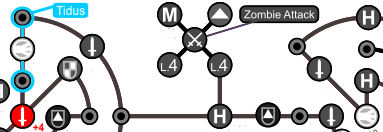
\includegraphics[width=.8\columnwidth]{graphics/tidus_bikanel}
\end{spheregrid}}{}
\begin{enumerate}[resume]
	\blitzballdetermination[true]{
		\item \formation{\tidus}{\lulu}{\auron}
	}{
		\item \formation{\tidus}{\rikku}{\kimahri}
	}
	\item You need 22 Power Spheres and 10 Speed Spheres \textbf{at this point} to be done farming them.
	\item At the bottom of the pit, \pickup{Teleport Spheres}
	\item Sandragora skip:
		\begin{itemize}
			\item Go near the Sandragora pit that blocks the entrance to Home
			\item Run North into the wall just on the right of the pit until Tidus is in the pit
			\item Let \rikku\ push you (don't move until she goes past you)
			\item Go north and enter Home
			\item If you fail the skip you can Flee and retry
		\end{itemize}
\end{enumerate}
\ \lossvfill \ \lossnewline \losscb \ 

    \chapter{Home}

\begin{enumerate}
    \item Go into door, \sd
\end{enumerate}
\begin{battle}{Bombs}
    \begin{itemize}
        \tidusf Haste \tidus
        \tidusf Attack each, starting with Guado
        \blitzballdetermination[true]{
            \item Others: Defend
        }{
            \rikkuf Grenade
            \kimahrif Lancet Bomb to refill OD, then switch to \auron\ and Defend
        }
    \end{itemize}
    Guaranteed 6 Power Spheres.
\end{battle}
\begin{enumerate}[resume]
    \item \sd
\end{enumerate}
\begin{battle}{Dual Horn}
    \begin{itemize}
        \switch{anyone}{\kimahri}
        \blitzballdetermination[true]{%
            \kimahrif Lancet Dual Horn (Fire Breath) if he doesn't have \od
        }{}
        \kimahrif \od\ Stone Breath
    \end{itemize}
\end{battle}
\begin{enumerate}[resume]
    \item Go down the stairs. Once the camera flips, \formation{\tidus}{\lulu}{\auron}
    \blitzballdetermination[true]{}{%
        \item Go back up the stairs into the left door.
        \item You will be forced into another Dual Horn encounter
        \begin{battle}{Dual Horns}
            \begin{itemize}
                \kimahrif Lancet Dual Horn (Fire Breath)
                \kimahrif \od\ Stone Breath
            \end{itemize}
        \end{battle}
        \item \formation{\tidus}{\lulu}{\auron}
        \item Open the right chest for a \textbf{Friend Sphere}, with the codes: Bottom Middle (up x2), Middle Right (up x4), Middle (down x4), exit the room and go down the stairs once again
	}
    \item Go left into the door, \cs[0:50]
\end{enumerate}
\begin{battle}{Chimera}
    \begin{itemize}
        \switch{anyone}{\kimahri}
        \kimahrif Lancet Chimera (Aqua Breath)
        \kimahrif \od\ Stone Breath
    \end{itemize}
\end{battle}
\winvfill
\begin{enumerate}[resume]
    \item Walk down steps, \cs[1:30]
    \item Before going further, \pickup{Level 2 Key Sphere} and \pickup{Level 4 Key Sphere}
    \item \sd\ until \tidus\ asks ``why'', \cs[6:20]
    \item \formation{\tidus}{\rikku}{\kimahri}
    \item Go bottom right to the next screen, run across the bridge
\end{enumerate}
    \chapter{Airship}

\begin{enumerate}
    \item \sd\ during \cs+3 \skippablefmv. Walk down corridor to the next screen, go back in, \sd. Speak to Brother, \sd. Walk towards corridor, \sd. Walk towards camera to the next screen, go up.
    \item If you need more than 4 Power Spheres or any Speed Spheres, buy Distillers from Rin, each one counts as 2 Spheres (need 28 Power Spheres and 10 Speed Spheres for the rest of the run).
    \item \save. Make sure that \rikku\ has \od. If she doesn't, you can get encounters on Rin's first screen.
\end{enumerate}
\begin{battle}[32000]{Evrae}
    Turns in this fight can be a bit random at times - Treat each character independantly of each other, doing their action as their turn comes up.
    \begin{itemize}
        \blitzballdetermination[true]{%
            \tidusf Haste \tidus
            \tidusf Cheer
            \tidusf If \tidus\ is still going next, immediately after his previous action, Change Weapon to Sonic Steel
            \rikkuf \od\ Mix Luck Sphere + Map
            \tidusf Attack x2
            \tidusf Cheer
            \tidusf Attack x3
            \item \kimahri\ or \rikku: Heal \tidus\ with an Elixir/X-Potion/Mega-Potion if he was hit in the first attack, Steal otherwise
        }{%
            \tidusf Haste \tidus
            \tidusf Cheer x2
            \tidusf Equip Baroque Sword [Strength +5\%, -]
            \tidusf Attack x6
            \rikkuf \od\ Mix Luck Sphere + Map
            \item \kimahri\ or \rikku: Heal \tidus\ with an Elixir/X-Potion/Mega-Potion, Lunar Curtain \tidus\ or Steal
        }
    \end{itemize}
\end{battle}
\begin{enumerate}[resume]
    \item \sd, \skippablefmv[3:00] - Press Start immediately after the FMV.
\end{enumerate}
    \chapter{Bevelle}
\begin{enumerate}
	\item Use a Mega-Potion
	\ifthenelse{\equal{\blitzresult}{win}}{}{
		\ifthenelse{\equal{\blitzresult}{both}}{
			\item \textit{If you \lostblitz:}
	}{}
		\begin{equip}
			\begin{itemize}
				\tidusf Equip Sonic Steel
			\end{itemize}	
		\end{equip}
	}
	\item \textit{With Sleeping Powder:}
\end{enumerate}
\begin{battle}{Guard Fights - Sleeping Powder}
	\begin{itemize}
		\item \textit{Fights 1 and 3 (3 Monks):}
			\begin{itemize}
				\tidusf Attack
				\item Others: Defend or use Distillers
			\end{itemize}
		\item \textit{Fights 2 and 4 (2 Monks and a YKT-63):}
			\begin{itemize}
				\tidusf Attack the YKT-63
				\rikkuf Sleeping Powder
				\kimahrif Smoke Bomb/Silence Grenade/Sleeping Powder
				\blitzballdetermination[true]{}{%
					\item \textit{If the YKT-63 is still alive} Use a Lightning Marble/Arctic Wind/Fish Scale or Attack with \tidus
				}
			\end{itemize}
		\item \textit{Fight 5 (2 Monks and a YAT-99):}
			\begin{itemize}
				\item \textit{If you have 2 Smoke Bombs/Sleeping Powders/Silence Grenades:}
					\begin{itemize}
						\tidusf Haste \rikku
						\rikkuf Sleeping Powder/Smoke Bomb/Silence Grenade
						\rikkuf If the Guards are sleeping use a Bomb Core on the YAT-99
						\rikkuf Sleeping Powder/Smoke Bomb/Silence Grenade
						\tidusf Attack
					\end{itemize}
				\item \textit{If you have 2 Bomb Cores:}
					\begin{itemize}
						\tidusf Attack the Monks
						\item Others: Use Bomb Core x2 on the YAT-99
					\end{itemize}
			\end{itemize}
	\end{itemize}
\end{battle}
\bothvfill
\lossvfill
\winvfill
\ 
\bothcb
\wincb
\losscb
\ 
\ \bothnewline \winnewline \lossnewline
\begin{enumerate}[resume]
	\item \textit{Without Sleeping Powder:}
		\begin{itemize}
			\item Keep \formation{\tidus}{\rikku}{\lulu} for the first 4 fights, \formation{\tidus}{\rikku}{\kimahri} for the last one
		\end{itemize}
\end{enumerate}
\begin{battle}{Guard Fights - No Sleeping Powder}
	\begin{itemize}
		\item \textit{Fights 1 and 3 (3 Monks):}
			\begin{itemize}
				\tidusf Attack
				\item Others: Defend or use Distillers
			\end{itemize}
		\item \textit{Fights 2 and 4 (2 Monks and a YKT-63):}
			\begin{itemize}
				\switch{\tidus}{\kimahri}
				\kimahrif Silence Grenade/Smoke Bomb
				\rikkuf Silence Grenade/Smoke Bomb
				\switch{\kimahri}{\tidus}
				\tidusf Attack the YKT-63
				\blitzballdetermination[true]{}{%
					\item \textit{If the YKT-63 is still alive} Use a Lightning Marble/Arctic Wind/Fish Scale or Attack with \tidus
				}
			\end{itemize}
			\item \textit{Fight 5 (2 Monks and a YAT-99):}
			\begin{itemize}
				\item \textit{If you have 2 Smoke Bombs/Silence Grenades:}
					\begin{itemize}
						\tidusf Haste \rikku
						\rikkuf Smoke Bomb/Silence Grenade x2
						\tidusf Attack
					\end{itemize}
				\item \textit{If you have 2 Bomb Cores:}
					\begin{itemize}
						\tidusf Attack the Monks
						\item Others: Use Bomb Core x2 on the YAT-99
					\end{itemize}
			\end{itemize}
	\end{itemize}
\end{battle}
\begin{enumerate}[resume]
	\item \sd, \skippablefmv[1:30], \sd\ on \yuna\ dialogue. \skippablefmv[30], \sd. Use lift, \sd.
\end{enumerate}
\bothvfill
\winvfill
\lossvfill
\ 
\begin{trial}
	\begin{itemize}
		\item \textit{Upper section:}
			\begin{itemize}
				\item Push the pedestal in
				\item Press X
				\item Go left at the 2nd junction
				\item Take sphere, push pedestal back
				\item At the 3rd junction, go back (hold X)
				\item Go left at the 2nd junction
				\item Place sphere into wall, push pedestal back
				\item At the 3rd junction, go back (hold X)
				\item Go left at the 1st junction
			\end{itemize}
		\item \textit{Lower section (1st visit):}
			\begin{itemize}
				\item The platform will automatically stop at the 1st junction
				\item After the platform stops, press X the 2nd time the arrow is pointing left
				\item Go right at the 3rd junction (hold X after the 2nd junction)
				\item Take Glyph sphere from wall, push pedestal back
				\item At the 4th junction go right (hold X)
				\item Place Glyph sphere into pedestal
				\item Take Bevelle sphere from pedestal
				\item Place Bevelle sphere into the wall
				\item Take the Glyph sphere
				\item Place Glyph sphere into the next wall
				\item Take Destruction sphere from the new wall
				\item Place Destruction sphere on the pedestal
				\item Take Bevelle sphere from the wall
				\item Push pedestal back and fall off the edge
			\end{itemize}
		\item \textit{Lower section (2nd visit):}
			\begin{itemize}
				\item Go straight (hold X)
				\item At the 3rd junction go right (hold X after the 2nd junction)
				\item Place Bevelle sphere on the pedestal
				\item Take Destruction sphere from the pedestal
				\item Place Destruction sphere into wall
				\item Push pedestal back and fall off the edge
			\end{itemize}
		\item \textit{Lower section (3nd visit):}
			\begin{itemize}
				\item Go straight
				\item At the 2nd junction go right (hold X)
				\item Push pedestal
				\item Go up the stairs, open the chest
			\end{itemize}
	\end{itemize}
\end{trial}
\begin{enumerate}[resume]
	\item \sd, name \bahamut, don't save, \sd
\end{enumerate}
\lossvfill
\ 
\losscb
\ \lossnewline \ 

    \chapter{Via Purifico}

\begin{enumerate}
	\item Run up past the first telepad
	\item Go to the second telepad and travel north.
\end{enumerate}
\bothvfill
\winvfill
\begin{spheregrid}
	\begin{itemize}
		\auronf
		\begin{itemize}
			\item Move $\rightarrow\rightarrow\rightarrow$
			\item Level 2 Keysphere
			\item Move $\rightarrow\rightarrow\rightarrow\rightarrow$
			\item Level 2 Keysphere
			\item Move $\uparrow\uparrow$
			\item Mag+3
		\end{itemize}
		\ifthenelse{\equal{\colstyle}{multi}}{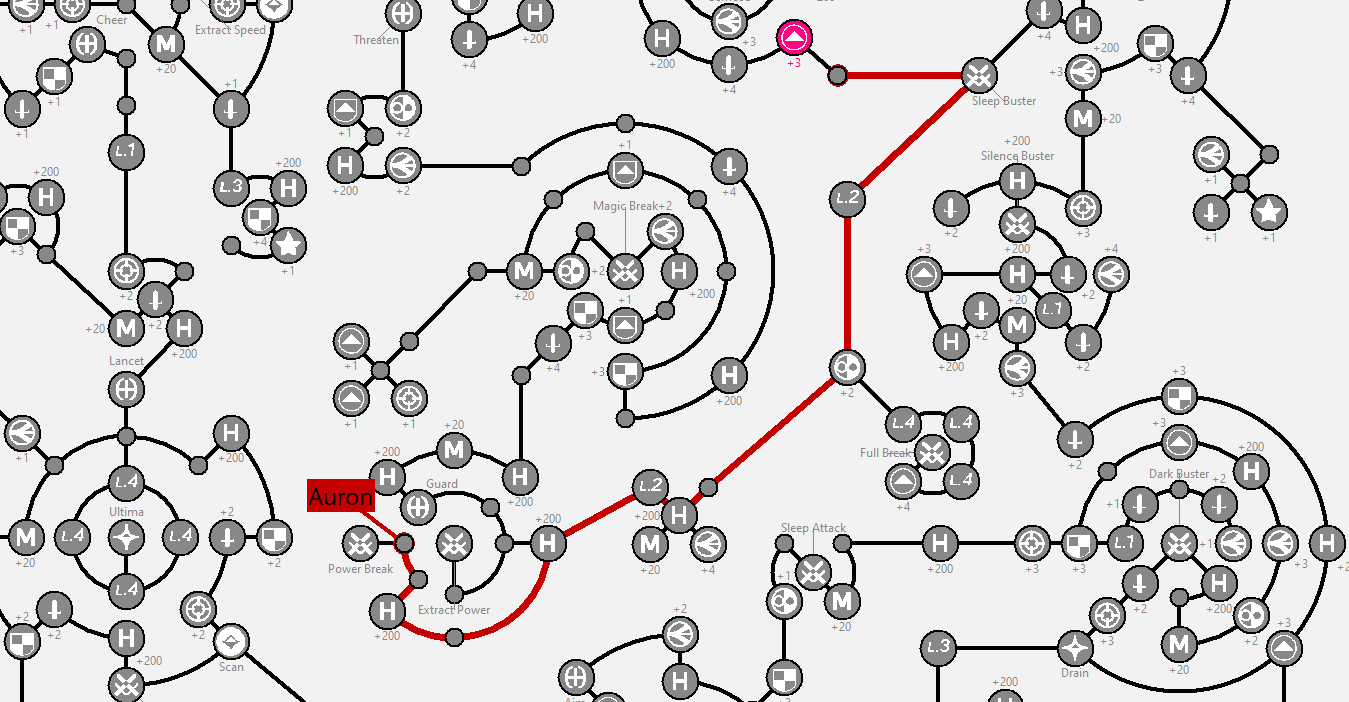
\includegraphics[width=.8\columnwidth]{graphics/Auron_Via_Purifico}}{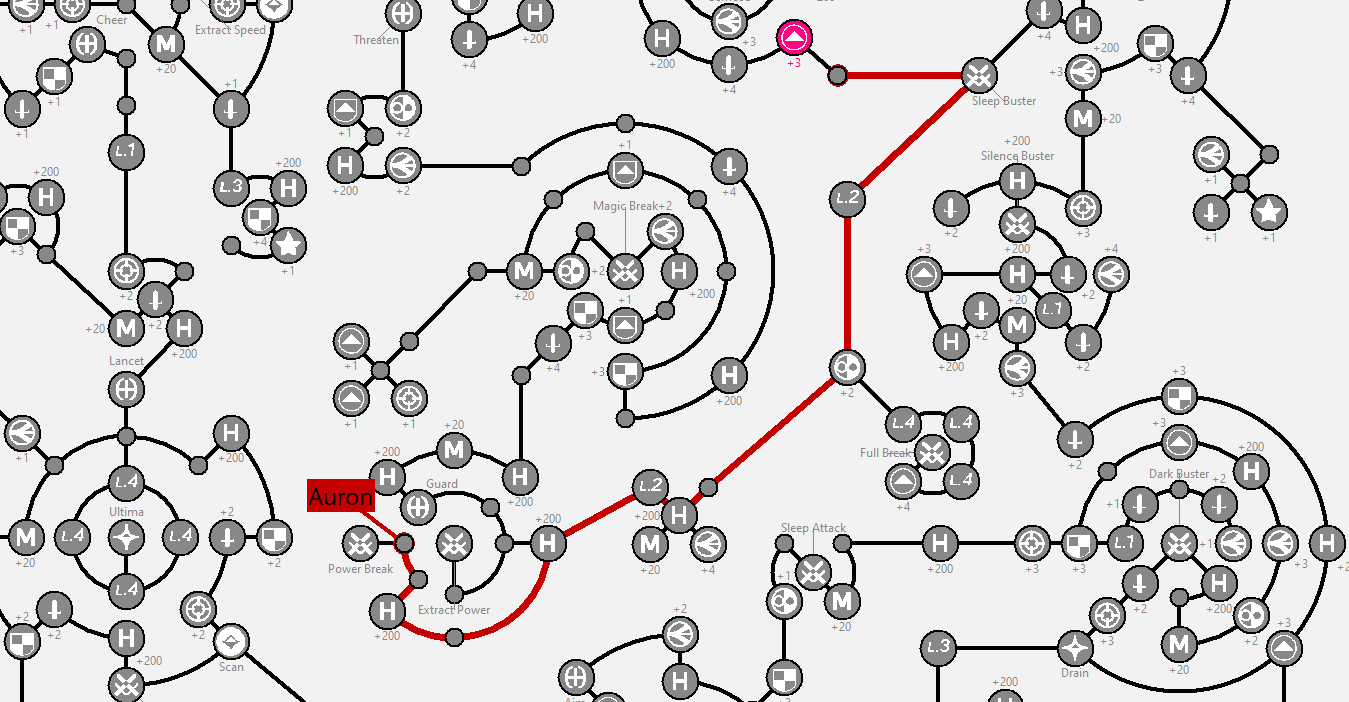
\includegraphics[width=.45\columnwidth]{graphics/Auron_Via_Purifico}}
		\yunaf
		\begin{itemize}
		\begin{multicols}{2}
			\item Move $\uparrow\uparrow$
			\item Level 4 Keysphere
			\item Move $\rightarrow\rightarrow\rightarrow\rightarrow\leftarrow$
			\item Str+2, Str+2, Str+2
			\item Teleport Sphere to \auron's Magic Node $\uparrow$
			\item Use Magic Sphere
			\item Str+4, Mag+3, Mag+4
			\item Move $\rightarrow\rightarrow\rightarrow\uparrow$
			\item Mag+3, HP+200, Str+4
			\item Move $\rightarrow$
			\item Def+3, Str+4
			\item Move $\leftarrow\downarrow$
			\item Agi+3, MP+20
			\item Move $\leftarrow\downarrow$
			\item HP+200, Str+2
			\item Move $\downarrow\downarrow$
			\item Str+2, Mag+3
			\item Level 1 Keysphere
			\item Move $\searrow\searrow$
			\item Agi+4, Str+2
			\item Move $\leftarrow\leftarrow$
			\item Str+2
			\item Move $\downarrow$
			\item Str+2, MP+20, Agi+3
			\end{multicols}
		\end{itemize}
		\ifthenelse{\equal{\colstyle}{multi}}{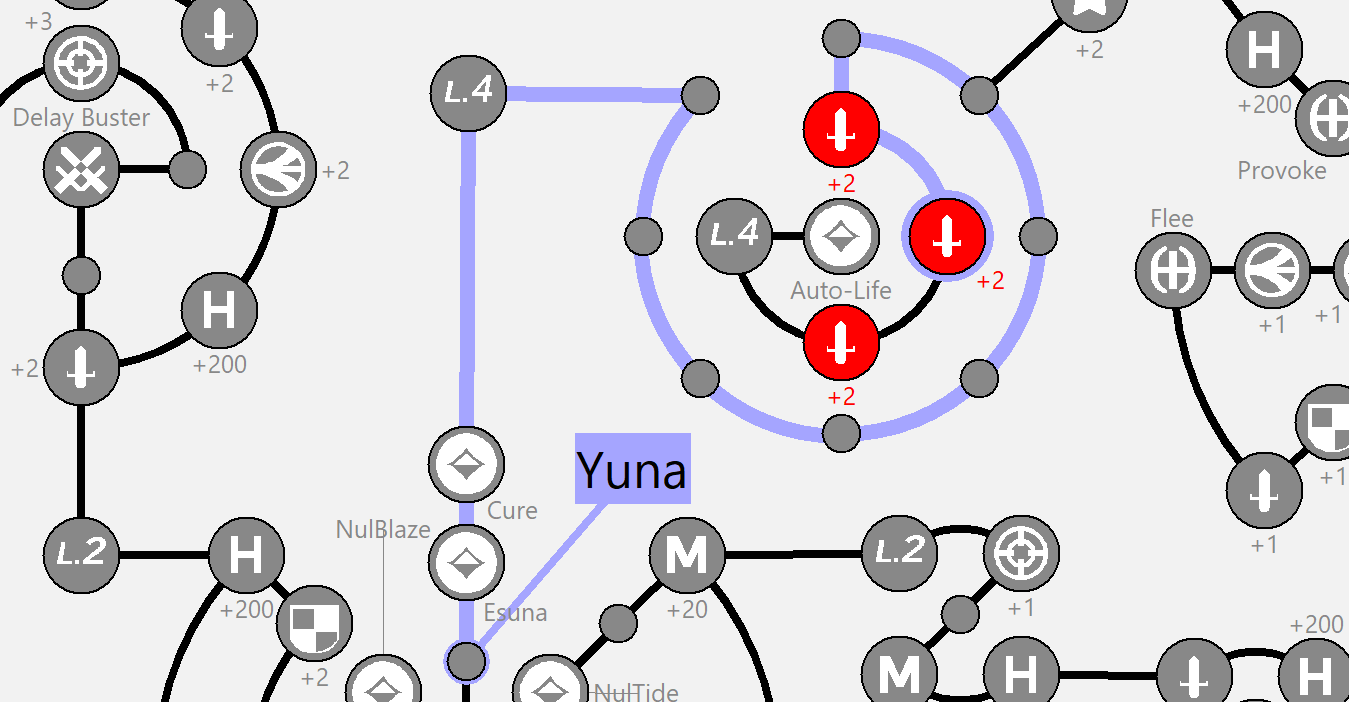
\includegraphics[width=.8\columnwidth]{graphics/via_purifico_yuna_1}}{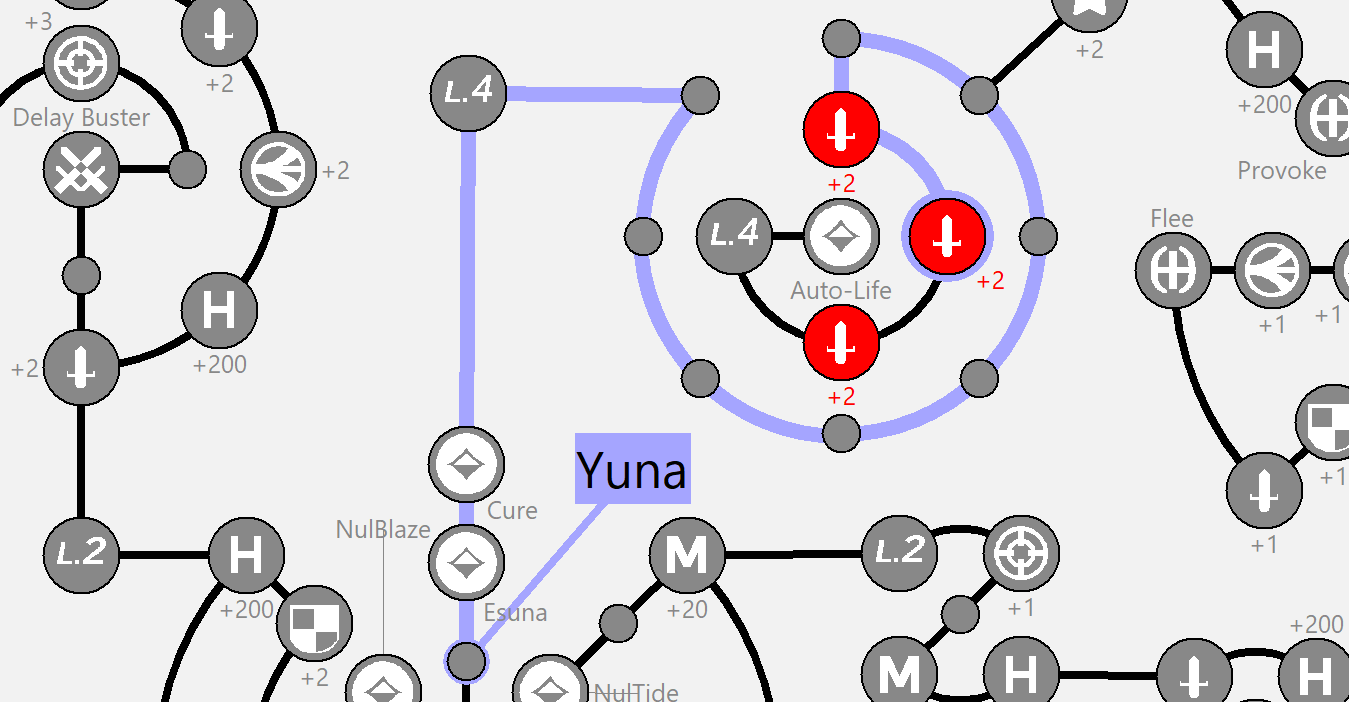
\includegraphics[width=.45\columnwidth]{graphics/via_purifico_yuna_1}}
		\ifthenelse{\equal{\colstyle}{multi}}{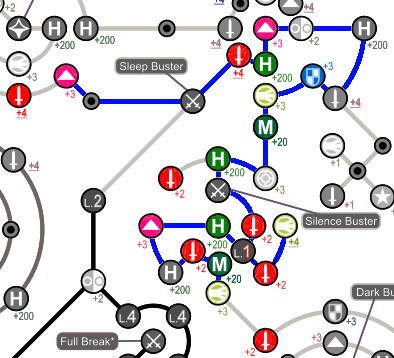
\includegraphics[width=.8\columnwidth]{graphics/via_purifico_yuna_2}}{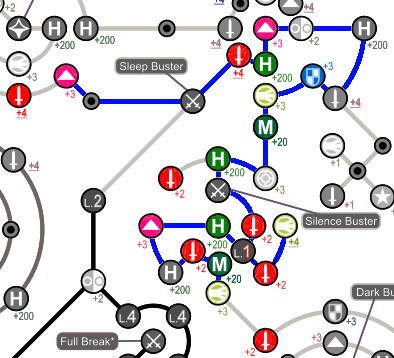
\includegraphics[width=.45\columnwidth]{graphics/via_purifico_yuna_2}}
	\end{itemize}
\end{spheregrid}
\begin{enumerate}[resume]
	\item You need 13 Power Spheres and 7 Speed Spheres for the rest of the run.
	\item \save
	\item Keep track of how many things you kill here.
\end{enumerate}
\begin{encounters}
	\begin{itemize}
		\item Maze Larva: Summon \ixion, Attack
	\end{itemize}
\end{encounters}
\bothvfill
\winvfill
\lossvfill
\begin{battle}{Isaaru}
	\begin{itemize}
		\item Grothia (8000 HP):
		      \begin{itemize}
			      \summon{\bahamut}
			      \bahamutf Attack
		      \end{itemize}
		\item Pterya (12000 HP):
		      \begin{itemize}
			      \summon{\bahamut}
			      \bahamutf Attack
		      \end{itemize}
		\item Spathi (20000 HP):
		      \begin{itemize}
			      \summon{\ixion}
			      \ixionf Attack x4
		      \end{itemize}
	\end{itemize}
\end{battle}
\begin{enumerate}[resume]
	\item Swim right and then up. Can use the underwater chest at the start to buy Power/Speed Distillers. If needed, you can attack Yellow Starfish and Sahagins with \tidus\ for 2x Power Spheres.
\end{enumerate}
\begin{battle}{Evrae Altana}
	\begin{itemize}
		\item Anyone: 1 Power/Speed Distiller if needed
		\item Anyone: Elixir/Phoenix Down x2 Evrae Altana
	\end{itemize}
\end{battle}
\begin{enumerate}[resume]
	\item Swim to exit, \sd
\end{enumerate}
\ 
\bothvfill
\ \bothnewline
\bothcb
\ 

\bothnpsingle
    \chapter{Highbridge}
\begin{spheregrid}
    \begin{itemize}
        \yunaf
        \blitzballSphereGrid{%
            \item Teleport to Strength Sphere $\uparrow\uparrow$ or $\nearrow$
            \item Str+4, Str+4, Def+3
            \item Move $\leftarrow\leftarrow$
            \item Str+4, HP+200, Agi+2
            \item Move $\rightarrow$
            \item Def +3
            \item Move $\leftarrow\leftarrow$
            \item Str+4
        }{.7}{.4}{graphics/Yuna_blitz_WIN_highroad}{%
            \item Teleport to \tidus\ Str+4 by Mental Break $\leftarrow$
            \item Str+4
            \item Friend Sphere to \tidus\ $\uparrow$
            \item Str+4, Agi+2
            \item Move $\rightarrow\rightarrow$
            \item Str+4
            \item Move $\rightarrow\rightarrow\rightarrow\rightarrow$
            \item Str+4
            \item Move $\rightarrow$
            \item Def+3
        }{.7}{.4}{graphics/Yuna_blitz_loss_highbridge_1}
    \end{itemize}
\end{spheregrid}
\begin{enumerate}
    \item \formation{\tidus}{\yuna}{\wakka}
    \item From this point on, watch any pre-empts if \yuna\ is in the party, because she will get the first turn. Check to make sure that \lulu\ has 35 levels.
    \item Need 4 Maze Larva/YKT-63 Kills total, Overkills count as 1.
    \item Walk north
\end{enumerate}
\begin{encounters}
    \begin{itemize}
        \item YKT-63:
        \begin{itemize}
            \tidusf Attack
            \yunaf Attack
            \item Flee
        \end{itemize}
    \end{itemize}
\end{encounters}
\begin{battle}[36000]{Seymour Natus}
    \begin{itemize}
        \item \textit{If \lulu\ has less than 35 levels:}
        \begin{itemize}
            \switch{\tidus}{\lulu}
            \luluf Switch Weapon
            \switch{\lulu}{\tidus}
        \end{itemize}
        \tidusf Attack
        \summon{\bahamut}
        \bahamutf Attack
    \end{itemize}
\end{battle}
\begin{enumerate}[resume]
    \item \sd
    \item Walk to \yuna, \cs+\skippablefmv[10:10]. Walk down, \cs[1:40], walk right, exit Macalania Woods
\end{enumerate}

    \chapter{Calm Lands}

\begin{enumerate}
	\item \sd, walk left
\end{enumerate}
\begin{spheregrid}
	\begin{itemize}
		\yunaf
		\blitzballSphereGrid{%
			\item Move $\leftarrow\leftarrow\leftarrow\leftarrow$
			\item Str+4
		}{.5}{graphics/yuna_blitz_win_calm_lands}{%
			\item Move $\leftarrow$
			\item HP+200, Str+4, Agi+2
		}{.5}{graphics/yuna_calm_land_loss}
	\end{itemize}
\end{spheregrid}
\begin{enumerate}[resume]
	\item \textit{If you have less than 2 \textbf{Water Gems}:} \formation{\tidus}{\yuna}{\kimahri}, then steal Gems from \textbf{Non-Ambush} Flame Flans until you have 2 total
\end{enumerate}
\begin{encounters}
	\begin{itemize}
		\item Flame Flan:
			\begin{itemize}
				\switch{anyone}{\rikku}
				\rikkuf Steal
				\switch{anyone}{\tidus}
				\item Flee
			\end{itemize}
	\end{itemize}
\end{encounters}
\begin{enumerate}[resume]
	\item \formation{\tidus}{\rikku}{\kimahri}
	\item Continue north to the Calm Lands Exit
	\item Run north, \sd
\end{enumerate}
\begin{battle}[64000]{Defender X}
	\begin{itemize}
		\switch{\tidus}{\yuna}
		\summon{\bahamut}
		\bahamutf Attack x2
	\end{itemize}
\end{battle}
\begin{enumerate}[resume]
	\item \sd, walk across bridge and up to Mt. Gagazet, \sd
\end{enumerate}
\lossvfill \winvfill
\ 
\losscb \wincb
\newline

    \chapter{Mt. Gagazet}
\begin{enumerate}
    \item Walk up, \cs[3:40], walk up, \sd
\end{enumerate}
\begin{battle}{Biran and Yenke}
    \begin{itemize}
        \kimahrif Steal from Biran
        \enemyf Biran Bulldoze
        \kimahrif Gem Yenke
        \kimahrif Gem Biran
    \end{itemize}
    Pay attention to your drops, they affect \yuna's sphere grid below.
\end{battle}
\begin{enumerate}[resume]
    \item The drop from the previous fight will give be one of the following:
        \begin{itemize}
            \item \textbf{4 Return Spheres}
            \item \textbf{2 Return Spheres and 2 Friend Spheres}
            \item \textbf{0 Return Spheres and 4 Friend Spheres}
        \end{itemize}
    \item These three branching paths will from now on be referred to by the number of \textbf{Return Spheres} that dropped.
\end{enumerate}
\bothvfill
\winvfill
\ \winnewline
\colend
\begin{spheregrid}
    \begin{multicols}{2}
        \begin{itemize}
            \luluf
            \begin{itemize}
                \item Move $\uparrow\uparrow$
                \item Level 2 Key Sphere
                \item Move $\downarrow x9$
                \item Level 3 Key Sphere
                \item Move $\searrow\searrow$
            \end{itemize}
            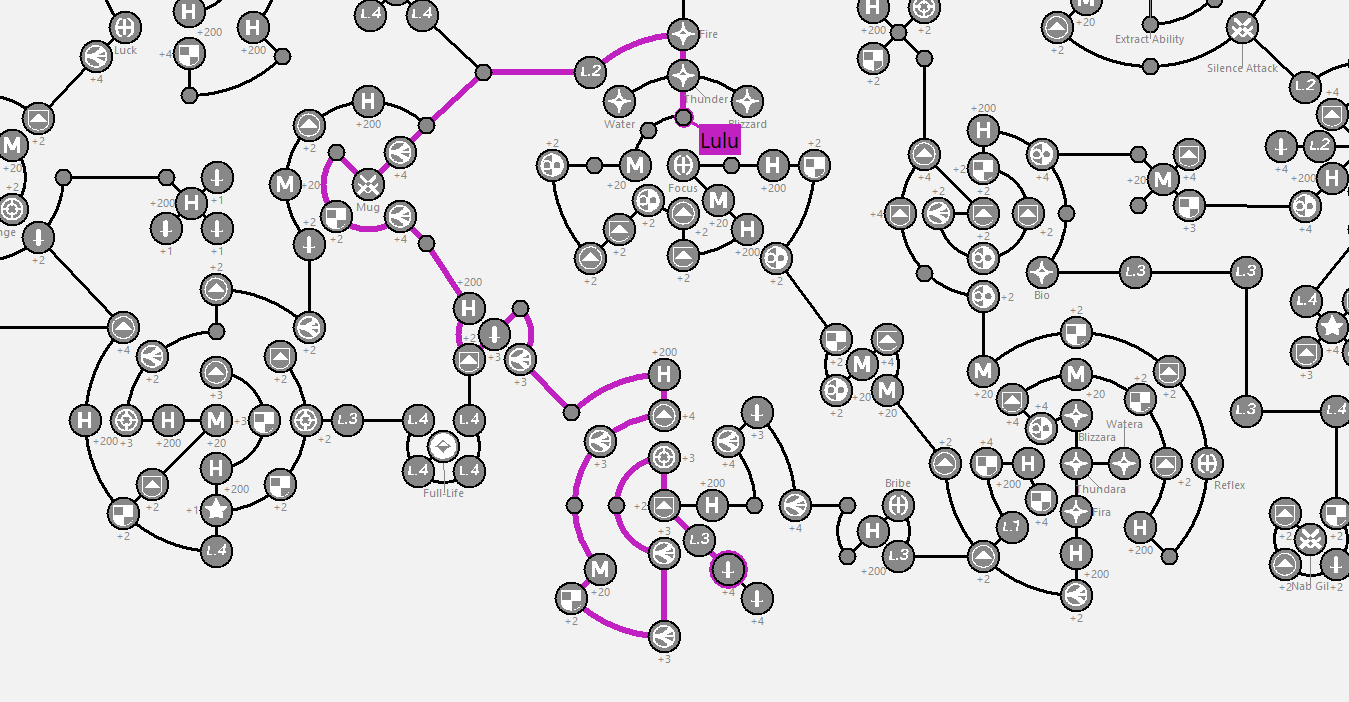
\includegraphics[width=.75\columnwidth]{graphics/lulu_grid}
            \yunaf
            \begin{itemize}
                \item \textit{If you got \textbf{4 Return Spheres}:}
                    \begin{itemize}
                        \item Use Return Sphere to Str+4 Node $\nwarrow$
                        \blitzballdetermination[true]{%
                            \item Move to the empty node $\leftarrow\downarrow$
                            \item Str+4, Agi+2
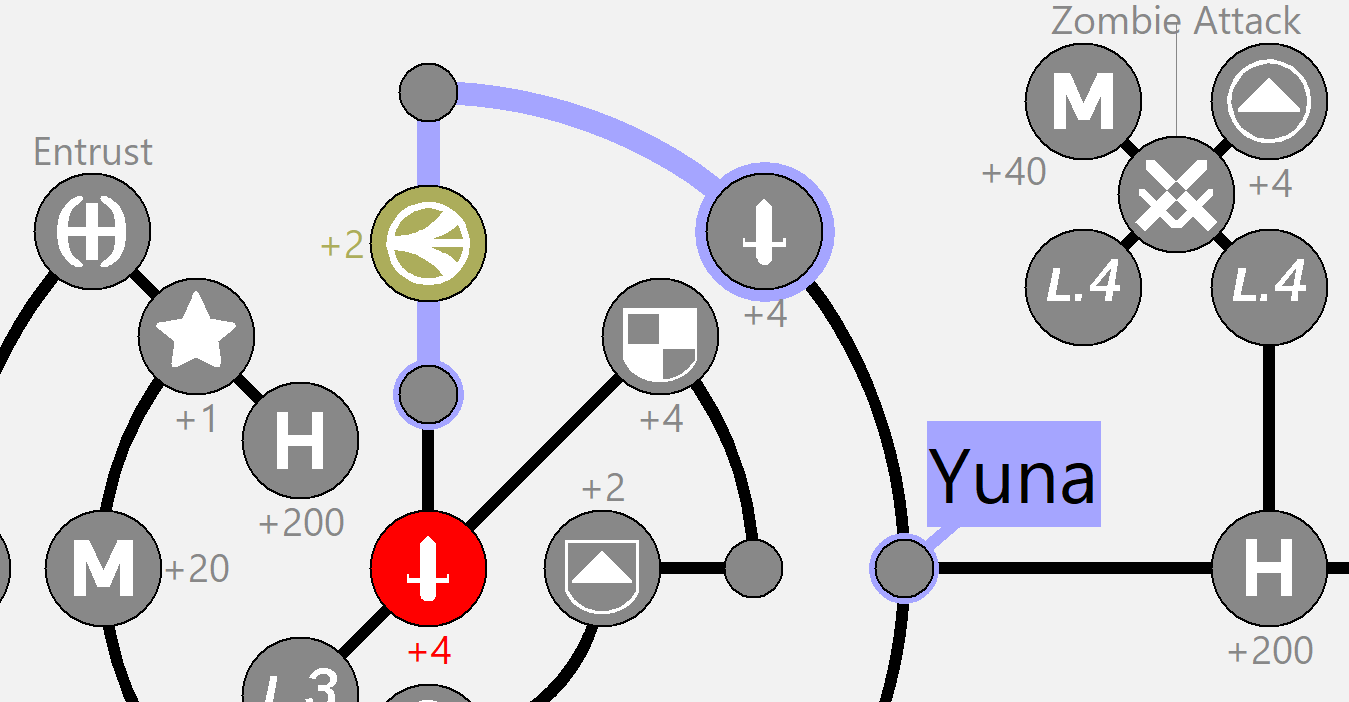
\includegraphics[width=.35\columnwidth]{graphics/4_returns_1}
                        }{%
                            \item Move to the empty node $\rightarrow\rightarrow\rightarrow$
                            \item Str+4, Def+3
                            \item 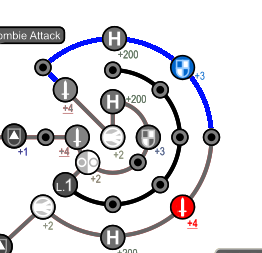
\includegraphics[width=.30\columnwidth]{graphics/loss_4_returns_1}
                        }
                    \end{itemize}
                
                \item \textit{If you got \textbf{2 Return Spheres}:}
                    \begin{itemize}
                        \blitzballdetermination[true]{%
                            \item Move to the empty node $\leftarrow$
                            \item Str+4, Agi+2
	                \item 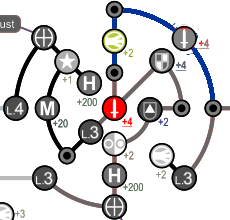
\includegraphics[width=.3\columnwidth]{graphics/2_and_2-1}
                        }{%
                            \item Move to the empty node $\rightarrow\rightarrow\rightarrow$
                            \item Str+4, Def+3
	                \item 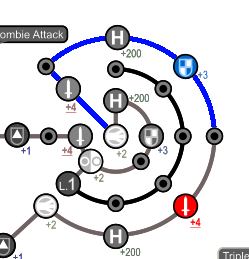
\includegraphics[width=.3\columnwidth]{graphics/loss_2_and_2-1}
                        }
                        \bothcb
                    \item Friend Sphere to \lulu, $\downarrow\downarrow$
                    \item Str+4, Str+4
                    \luluf Move $\nearrow\uparrow\uparrow$
                    \yunaf Friend Sphere to \lulu,
                    \item Str+3, Agi+4, Agi+4
                \end{itemize}
                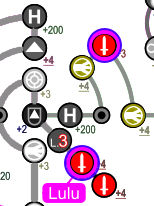
\includegraphics[width=.3\columnwidth]{graphics/2_and_2}
                \wincb
                \losscb
                \item \textit{If you got \textbf{0 Return Spheres}:}
                    \begin{itemize}
                        \kimahrif Move $\swarrow x2$
                        \blitzballdetermination[true]{
                            \tidusf Move to Str+4 by Mental Break $\rightarrow x3, \downarrow, \rightarrow x3$
                            \yunaf Move to the empty node $\leftarrow$
                            \yunaf Str+4, Agi+2
                        }{%
                            \tidusf Move to Armor Break $\rightarrow x3, \downarrow x6$
                            \tidusf Armor Break
                            \tidusf Move to HP $\searrow\searrow$
                            \item Move to the empty node $\rightarrow\rightarrow\rightarrow$
                            \item Str+4, Def+3
                        }
                        \yunaf Friend Sphere to \tidus
                        \yunaf Str+4
                        \item Friend Sphere to Lulu x2 like described \textbf{in the 2 Return Sphere Menu}
                        \yunaf Friend to \kimahri\ $\downarrow$
                        \yunaf Agi+4
                    \end{itemize}
                    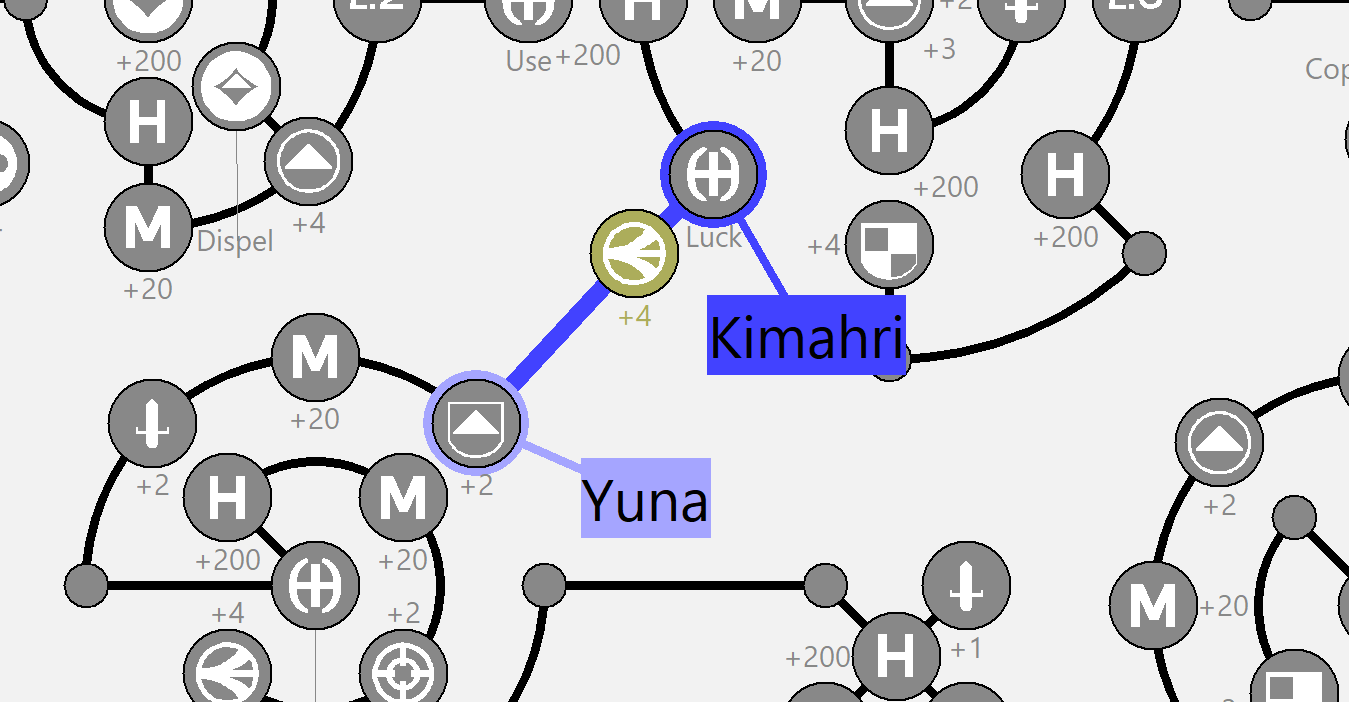
\includegraphics[width=.3\columnwidth]{graphics/post_BY_0_returns}
                    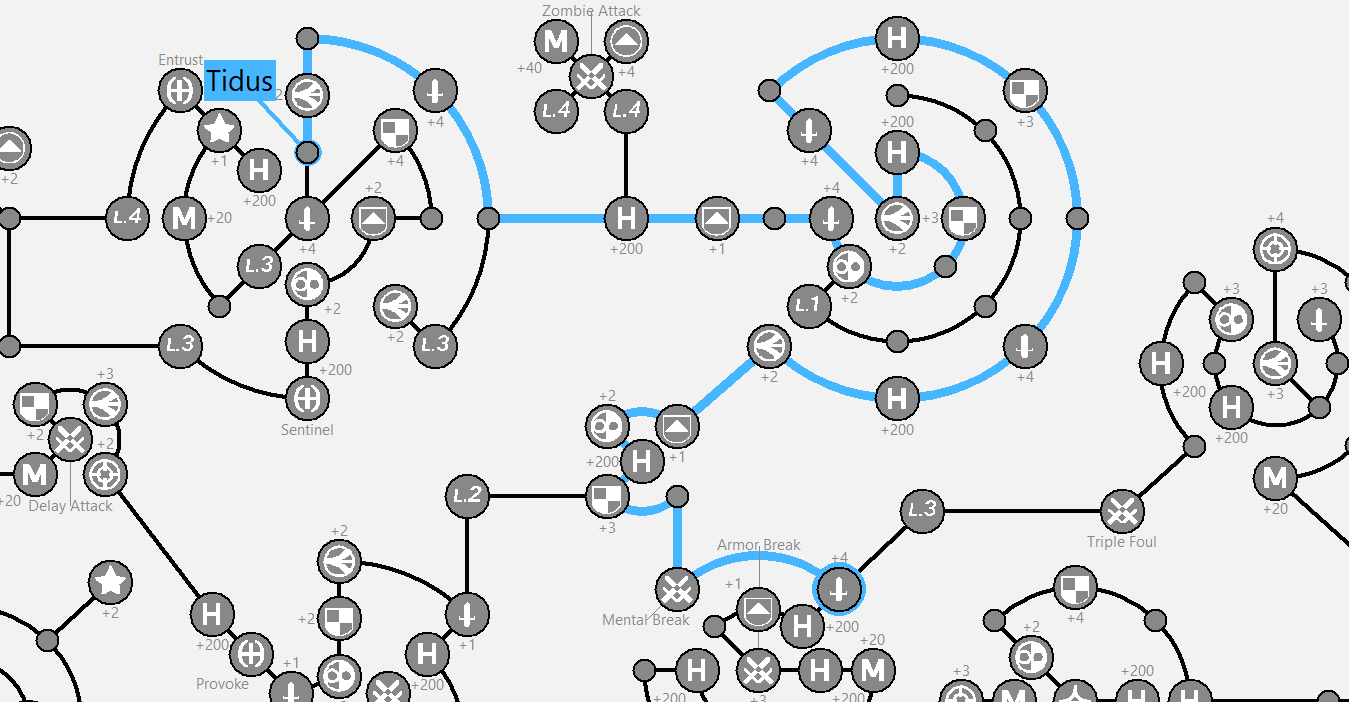
\includegraphics[width=.4\columnwidth]{graphics/0_returns_pt2}
            \end{itemize}
            \item \tidus\ \textit{if you didn't get Armor Break:}
                \begin{itemize}
                    \item \textit{If you got \textbf{4 Return Spheres}:}
                        \begin{itemize}
                            \item Move to Armor Break $\rightarrow x3, \downarrow x6$
                        \end{itemize}
                    \item \textit{If you got \textbf{2 Return Spheres}:}
                        \begin{itemize}
                            \item Return Sphere $\downarrow\searrow\searrow$, Str+4 near Armor Break
                            \item Move $\nwarrow\leftarrow$ or $\swarrow\swarrow$
                        \end{itemize}
                    \item \textit{If you got \textbf{0 Return Spheres}:}
                        \begin{itemize}
                            \item Move $\nwarrow\leftarrow$ or $\swarrow\swarrow$
                        \end{itemize}
                    \item Armor Break
                \end{itemize}
        \end{itemize}
    \end{multicols}
\end{spheregrid}
\colstart
\begin{enumerate}[resume]
    \item \textit{If you got \textbf{4 Return Spheres}:}
        \begin{itemize}
            \item Customize:
                \begin{itemize}
                    \auronf Shimmering Blade $\rightarrow$ First Strike
                    \yunaf Staff $\rightarrow$ First Strike
                \end{itemize}
        \end{itemize}
    \item \textit{If you got \textbf{2 Return Spheres}:}
        \begin{itemize}
            \item Customize:
            \begin{itemize}
                \yunaf Staff $\rightarrow$ First Strike
            \end{itemize}
        \end{itemize}
    \bothvfill
    \winvfill
    \lossvfill
    \item \textit{If you need need to charge \rikku's \od} \formation{\tidus}{\rikku}{\auron}, otherwise \formation{\tidus}{\kimahri}{\wakka}.
\end{enumerate}
\begin{enumerate}[resume]
    \item Walk up, \sd, \cs[1:20], continue walking up, avoid the gravestones.
    \item Charge \rikku's \od\ in an encounter with Mechs, Steal from the Mech Leader with \rikku\ and Escape with the others (optional if you have a Silence Grenade)
    \item Follow the path around.
    \item \textit{If you had 2 or 4 \textbf{Return Spheres}} \formation{\tidus}{\yuna}{\auron}, otherwise \formation{\tidus}{\kimahri}{\wakka}
\end{enumerate}
\begin{battle}[70000]{Seymour Flux}
    \begin{itemize}
        \item \textit{If you had 4 \textbf{Return Spheres}:}
            \begin{itemize}
                \yunaf Attack
                \tidusf Haste \yuna
                \switch{\auron}{\rikku}
                \rikkuf Silence Grenade or \od\ HP Sphere + Grenade
                \summon{\bahamut}
                \bahamutf \textit{If you used a Silence Grenade} Impulse, otherwise Attack
                \yunaf Attack
                \tidusf \textit{If you used a Silence Grenade} Attack once, otherwise Defend
                \rikkuf Defend
            \end{itemize}
        \item \textit{If you had 2 \textbf{Return Spheres}:}
            \begin{itemize}
                \yunaf Attack
                \tidusf Haste \yuna
                \summon{\bahamut}
                \bahamutf Impulse
            \end{itemize}        
        \item \textit{If you had 0 \textbf{Return Spheres}:}
            \begin{itemize}
                \switch{\tidus}{\yuna}
                \summon{\bahamut}
                \bahamutf Attack
            \end{itemize}
    \end{itemize}
\end{battle}
\begin{enumerate}[resume]
    \item \formation{\tidus}{\kimahri}{\auron}
    \item \save\ if \bahamut\ was banished, Walk to the next screen. \skippablefmv[0:20], \sd, walk up to \tidus\ House, go into the center, \sd. Follow the boy outside, speak to him upstairs, \sd.
    \item Walk up to the next screen, go up the steps. Go down the left path into the water, \sd, swim up. Go up the steps, play the minigame, return to the previous screen.
    \item \tidus\ can attack Splashers for Power Spheres (only attack the 3 fish group): if you got 4 \textbf{Return Spheres} you need 4 Power Spheres; if you got 2 or 0 \textbf{Return Spheres} you don't need any Power Spheres.
    \item Return to Save Sphere, go up and left, then go down the right path, swim up into the next screen. Complete the minigame, \rikku\ Green, \tidus\ Blue, \wakka\ Red. Return.
    \item Go up left path, \sd, continue up the path, \save\ if \bahamut\ was banished and you didn't touch one earlier.
    \item \formation{\tidus}{\yuna}{\wakka}. Go onto the next screen.
\end{enumerate}
\bothvfill
\winvfill
\lossvfill
\begin{battle}[40000]{Sanctuary Keeper}
    \begin{itemize}
        \item \textit{If you got 2 or 4 \textbf{Return Spheres}:}
            \begin{itemize}
                \yunaf Defend
                \tidusf Armor Break
            \end{itemize}
        \item \textit{If 0 \textbf{Returns Spheres}:}
            \begin{itemize}
                \tidusf Defend
            \end{itemize}
        \summon{\bahamut}
        \bahamutf Attack
    \end{itemize}
\end{battle}

    \chapter{Zanarkand}
\begin{enumerate}
    \item \sd, \cs[0:50], walk left. \fmv+\cs[2:20]
    \item Move left to the sphere, \sd, \cs[1:40]. Walk further left and follow the path down, \cs[3:20], walk left onto the next screen.
    \item \textit{If \rikku\ doesn't have \od} \formation{\tidus}{\auron}{\rikku}, otherwise \formation{\tidus}{\auron}{\kimahri}
    \item You can charge \rikku's \od\ on an encounter with a Behemoth or a Defender Z (Escape with the others).
    \item Open the first chest on the left for the \textbf{Fortune Sphere}, continue on the path until you get inside the Dome.
    \item If you got \textbf{4 Return Spheres} and you missed the Overkill on \textbf{Seymour Flux} kill two \textbf{YKT-11} or one \textbf{Defender Z} with \formation{\tidus}{\auron}{\yuna}, only \yuna\ needs the AP.
\end{enumerate}
\begin{encounters}
    \begin{itemize}
        \item YKT-11:
        \begin{itemize}
            \yunaf Attack
            \tidusf Attack
            \item Flee
        \end{itemize}
        \item Defender Z:
        \begin{itemize}
            \summon{\bahamut}
            \bahamutf Attack
        \end{itemize}
    \end{itemize}
\end{encounters}
\begin{enumerate}[resume]
    \item After Seymour's Mom \cs, if you had \textbf{4 Return Spheres} \pickup{Friend Sphere} on the right path.
    \item When you leave the last encounter zone, the hallway before the Zanarkand Trials, \pickup{Luck Sphere} on the right.
\end{enumerate}
\winvfill
\winnp
\lossvfill
\lossnp
\begin{spheregrid}
    \begin{itemize}
        \yunaf
        \begin{itemize}
            \item \textit{If you got \textbf{4 Return Spheres}:}
            \begin{itemize}
                \yunaf Friend Sphere to \lulu\ $\downarrow\downarrow$
                \item Str+4, Str+4
                \item Move $\nearrow$ to the empty node between HP+200 and Agi+4
                \item Agi+4
                \item Luck Sphere, Fortune Sphere
                \item Return Sphere to the Agi+4 node you just activated
                \item Str+3
                \item Return Sphere to the Str+3 node you just activated
                \item Agi+4
            \end{itemize}
            \ifthenelse{\equal{\colstyle}{multi}}{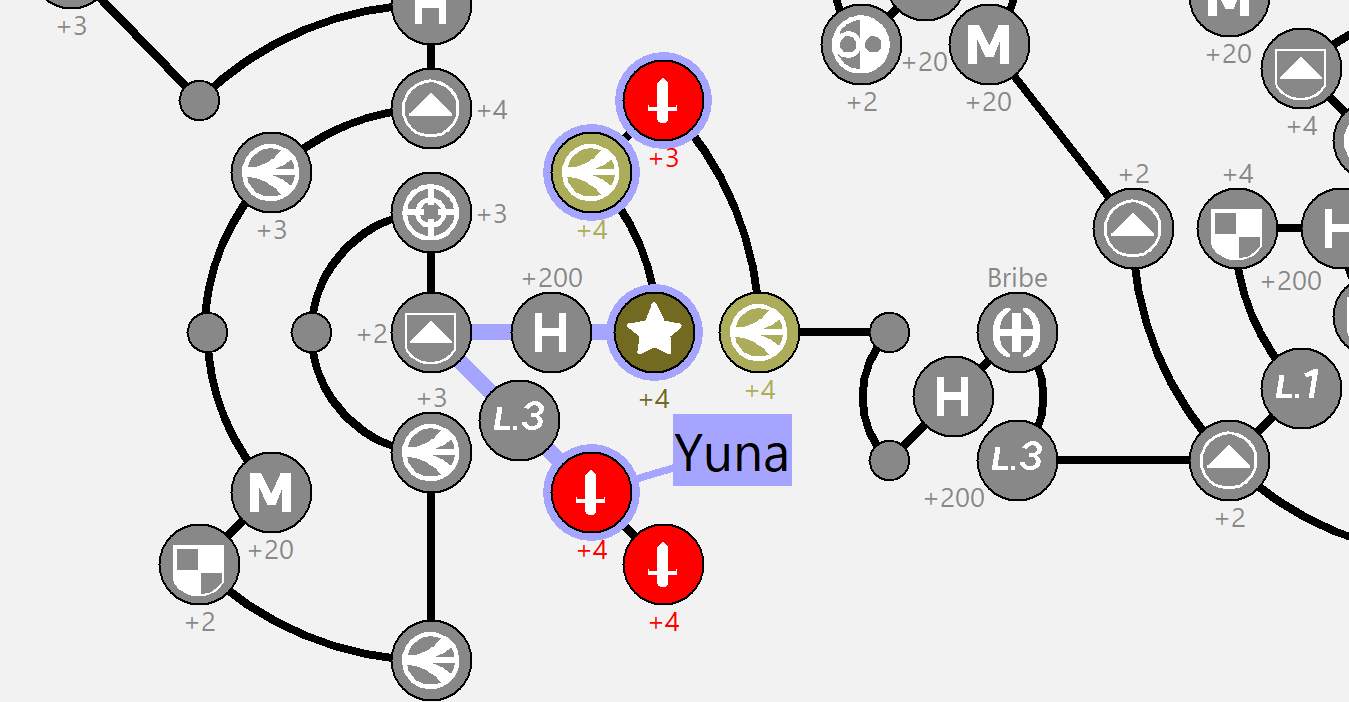
\includegraphics[width=.5\columnwidth]{graphics/4_returns_w_luck_pt1}}{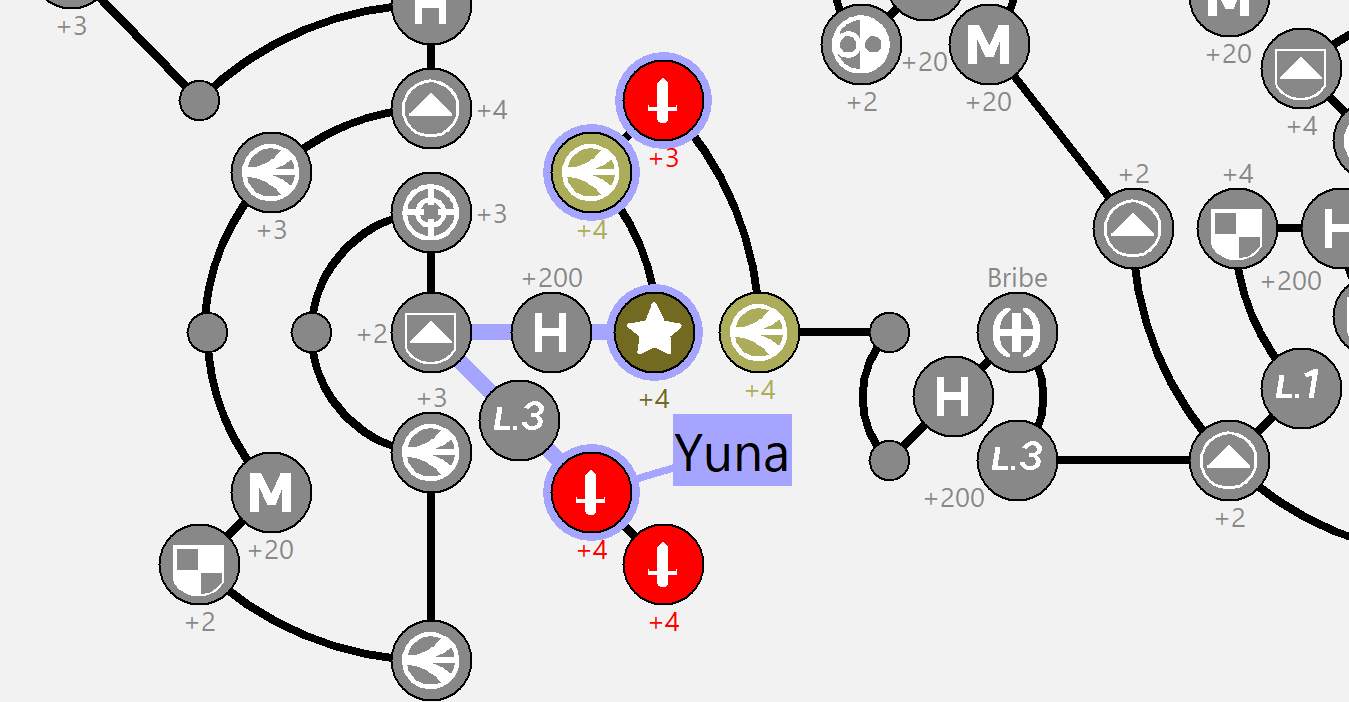
\includegraphics[width=.2\columnwidth]{graphics/4_returns_w_luck_pt1}}
            \item \textit{If you got \textbf{2 Return Spheres}:}
            \begin{itemize}
                \yunaf Use Blk Mag Sphere on Fire $\leftarrow\uparrow$
                \item Return Sphere to Fire $\uparrow$
                \item Move $\leftarrow\leftarrow\leftarrow$
                \item Luck Sphere, Fortune Sphere
                \item Agi+4
                \item Move $\downarrow\downarrow\downarrow\downarrow\leftarrow$
                \item MP+20, Str+2
            \end{itemize}
            \ifthenelse{\equal{\colstyle}{multi}}{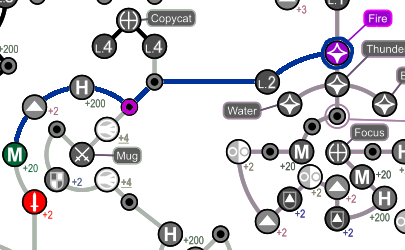
\includegraphics[width=.5\columnwidth]{graphics/2_and_2_with_luck}}{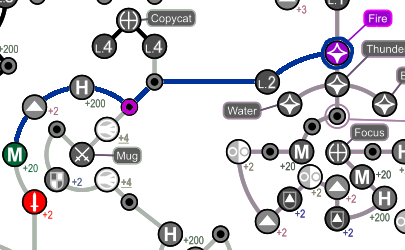
\includegraphics[width=.2\columnwidth]{graphics/2_and_2_with_luck}}
            \item \textit{If you got \textbf{0 Return Spheres}:}
            \begin{itemize}
                \yunaf Move $\swarrow\swarrow$
                \item Luck Sphere, Fortune Sphere, Spare Change
            \end{itemize}
            \ifthenelse{\equal{\colstyle}{multi}}{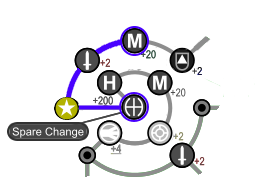
\includegraphics[width=.7\columnwidth]{graphics/0_return_w_luck}}{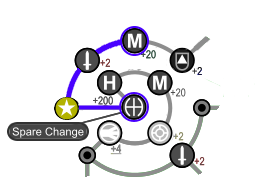
\includegraphics[width=.25\columnwidth]{graphics/0_return_w_luck}}
        \end{itemize}
    \end{itemize}
\end{spheregrid}
\bothcb \wincb \losscb
\begin{enumerate}[resume]
    \item \formation{\tidus}{\auron}{\yuna}
    \item \textit{If you had 0 Return Spheres:}
    \begin{itemize}
        \item Customize:
        \begin{itemize}
            \auronf Shimmering Blade $\rightarrow$ First Strike
            \yunaf Staff $\rightarrow$ First Strike
        \end{itemize}
    \end{itemize}
\end{enumerate}
\begin{enumerate}[resume]
    \item {\large \save}
\end{enumerate}
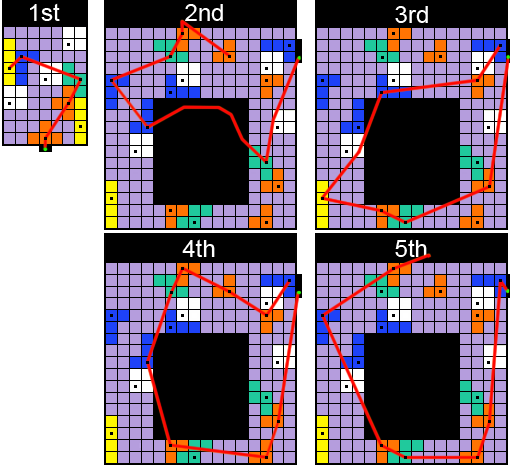
\includegraphics[width=.95\columnwidth]{graphics/Zanarkand_Trials}
\begin{enumerate}[resume]
    \item Push in the pedestals starting from the Top Left, to Bottom Left, then Top Right, Bottom Right, then Besaid Sphere. After pushing in each pedestal, do the corresponding puzzle, shown above.
    \item After the second puzzle, take the Kilika Sphere on the left and put it into the second pedestal.
    \item After the fifth puzzle, take the Besaid Sphere from the right and put it into the fifth pedestal.
    \item \cs, run into the large room
\end{enumerate}
\begin{battle}[52000]{Spectral Keeper}
    \begin{itemize}
        \summon{\bahamut}
        \bahamutf Attack x2
    \end{itemize}
\end{battle}
\bothvfill\winvfill\lossvfill
\begin{spheregrid}
    \begin{itemize}
        \item \textit{If you had 4 \textbf{Return Spheres}:}
        \begin{itemize}
            \item Use Blk Mag Sphere on Fire
            \item Return Sphere to Fire
            \item Move $\leftarrow\leftarrow\leftarrow$
            \item Agi+4
            \item Move $\leftarrow\leftarrow\leftarrow$
            \item MP+20, Str+2
        \end{itemize}
    \end{itemize}
    \ifthenelse{\equal{\colstyle}{multi}}{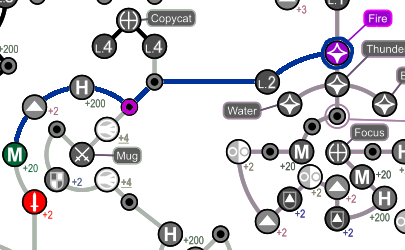
\includegraphics[width=.5\columnwidth]{graphics/2_and_2_with_luck}}{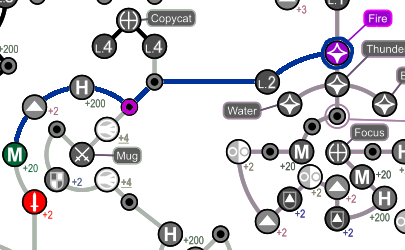
\includegraphics[width=.25\columnwidth]{graphics/2_and_2_with_luck}}
\end{spheregrid}
\begin{enumerate}[resume]
    \item \save, Run up, \sd\ by mashing another button (like \textbf{R1}) at the same time as confirm, walk up to Yunalesca's room, \sd
\end{enumerate}
\begin{battle}[132000]{Yunalesca}
    \begin{itemize}
        \summon{\bahamut}
        \bahamutf Attack x3
    \end{itemize}
    If any weapon drops, it will have \textbf{Zombie Strike}
\end{battle}
\begin{enumerate}[resume]
    \item \sd, leave room, walk down steps, \sd, go down on the next screens, \save, go up the lift, walk out of the cloister of trials, walk down the steps, walk down, \sd\ during \cs+\skippablefmv
\end{enumerate}
    \chapter{Airship}
\begin{enumerate}
	\item \sd, walk out of the cockpit past Rin, along the corridors to \yuna\ and \kimahri. \sd. Walk back to the cockpit, \sd. Talk to Cid to travel to Highbridge.
	\item Walk up to the Bevelle entrance, \sd. In the Fayth room, pick the \nth{1} option ``I Think So'', then pick the \nth{2} option ``Defeat Yu Yevon''
	\item Walk up to Cid, travel to Sin, \sd, \skippablefmv, \sd. Go through the corridors to the outside of the airship, \sd, 3 \skippablefmv[2:10], \sd
\end{enumerate}
\begin{battle}[65000]{Sin Left Fin}
	\begin{itemize}
		\summon{\bahamut}
		\bahamutf Impulse x2
	\end{itemize}
\end{battle}
\begin{enumerate}[resume]
	\item \sd, \cs+\skippablefmv
\end{enumerate}
\begin{battle}[65000]{Sin Right Fin}
	\begin{itemize}
		\summon{\bahamut}
		\bahamutf Impulse x2
	\end{itemize}
\end{battle}
\begin{enumerate}[resume]
	\item \sd, \cs+\skippablefmv
\end{enumerate}
\begin{battle}[56000]{Sin Genais and Core}
	\begin{itemize}
		\summon{\bahamut}
		\item \textit{If you still need Return Spheres:}
			\begin{itemize}
				\bahamutf Attack Genais
			\end{itemize}
		\bahamutf Impulse Core
	\end{itemize}
	Check for any weapon drops with \textbf{Zombie Strike} if you killed Genais.
\end{battle}
\begin{enumerate}[resume]
	\item \sd, \skippablefmv
	\item Walk along the corridors to the outside of the ship, speak to \yuna. \cs[1:40], \sd\ \rikku\ dialogue. \skippablefmv. Go through the corridors, go outside again, \skippablefmv, \sd.
\end{enumerate}
\begin{battle}[140000]{Overdrive Sin}
	\begin{itemize}
		\summon{\bahamut}
		\bahamutf Impulse
		\bahamutf Attack x2
	\end{itemize}
\end{battle}
\begin{enumerate}[resume]
	\item \skippablefmv[1:20], \sd
\end{enumerate}
    \chapter{Inside Sin}
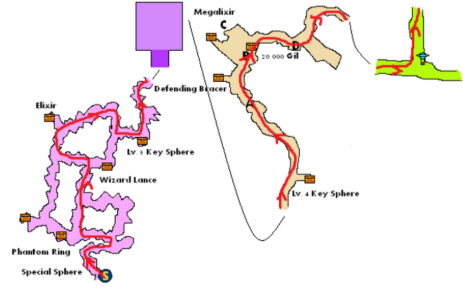
\includegraphics{graphics/sinpath}
\begin{enumerate}
    \item \textit{If \rikku\ doesn't have \od} \formation{\tidus}{\auron}{\rikku}, otherwise \formation{\tidus}{\auron}{\kimahri}
    \item Walk along the path, you can charge \rikku's \od\ on an encounter with a Behemoth King or Adamantoise (Escape with the others), flee from the rest.
    \item Before Seymour Omnis, \formation{\tidus}{\auron}{\yuna}
    \item \textit{If you got \textbf{2 Return Spheres}:}
    \begin{itemize}
        \item Customize:
        \begin{itemize}
            \auronf Shimmering Blade $\rightarrow$ First Strike
        \end{itemize}
    \end{itemize}
    \item Go up the steps, \sd
\end{enumerate}
\bothvfill\winvfill\lossvfill
\begin{battle}[80000]{Seymour Omnis}
    \begin{itemize}
        \yunaf Defend
        \tidusf Armor Break
        \item \textit{If Armor Break Hit:}
        \begin{itemize}
            \auronf Defend
        \end{itemize}
        \item \textit{If Armor Break Missed:}
        \begin{itemize}
            \switch{\auron}{\rikku}
            \rikkuf \od\ Mix Arctic Wind/Lightning Marble/Bomb Core/Fish Scale + HiPot/MegaPot/XPot/Mega Phoenix
            \yunaf Cure Mortiphasm
            \enemyf Firaga x3, Blizzara
            \yunaf Change Weapon to Wind Rod
            \tidusf Armor Break
        \end{itemize}
        \summon{\bahamut}
        \bahamutf Attack
    \end{itemize}
\end{battle}
\begin{enumerate}[resume]
    \item \sd, walk north.
    \item \formation{\tidus}{\kimahri}{\auron}
    \item You can charge \rikku's \od\ on an encounter with a Behemoth King, Adamantoise or Barbatos (Escape with the others), flee from the rest.
    \item Turn left onto the bridge, go onto the next screen.
    \item Complete the minigame, picking up the eggs and avoiding the crystals.
\end{enumerate}
\bothvfill\winvfill\lossvfill
\ 
\colend
\begin{spheregrid}
    \begin{multicols}{2}
        \begin{itemize}
            \item \textit{If you got 2 or 4 \textbf{Return Spheres}:}
            \begin{itemize}
                \item Move $\downarrow\downarrow$
                \item Agi+2
                \item Move $\leftarrow x5$
                \item Agi+4 (be careful to not activate the Acc+2 Node)
                \item Move $\nwarrow$
                \item Spare Change
                \item Attribute Sphere \kimahri's +4 Agi
            \end{itemize}
            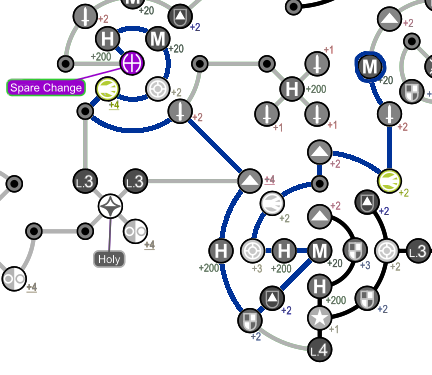
\includegraphics[width=.8\columnwidth]{graphics/4_Return_final_grid}
            \item \textit{If you got 0 \textbf{Return Spheres}:}
            \begin{itemize}
                \item Attribute Sphere \rikku's +3 Agi $\rightarrow$
                \item Spare Change
                \item Move $\downarrow$
                \item Agi+4 (be careful to not activate the Acc+2 Node)
                \item Move $\rightarrow x6$
                \item Agi+4
            \end{itemize}
            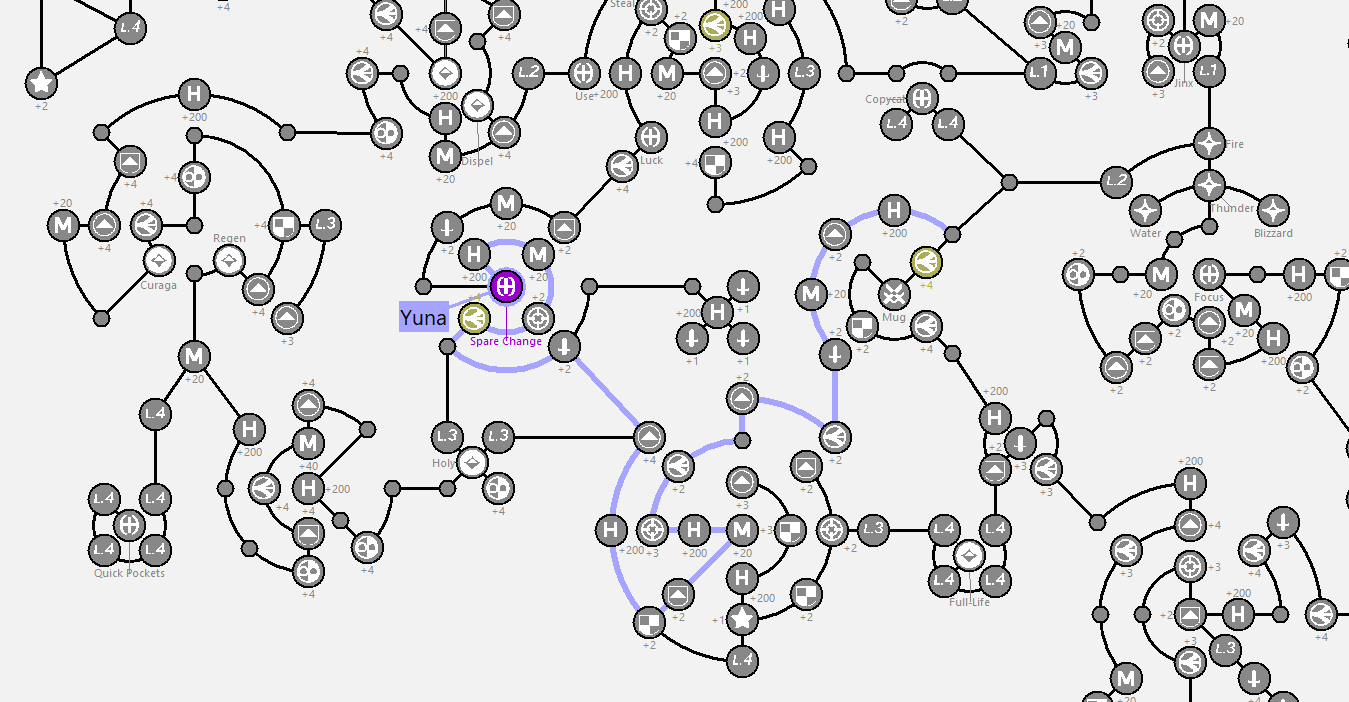
\includegraphics[width=.8\columnwidth]{graphics/0_return_before_BFA}
            \columnbreak
            \tidusf \textit{If you didn't get a \textbf{Zombie Strike} weapon}:
            \begin{itemize}
                \item Move $\uparrow x5$
                \item Level 4 Keysphere
                \item Move $\uparrow$
                \item Zombie Attack
            \end{itemize}
            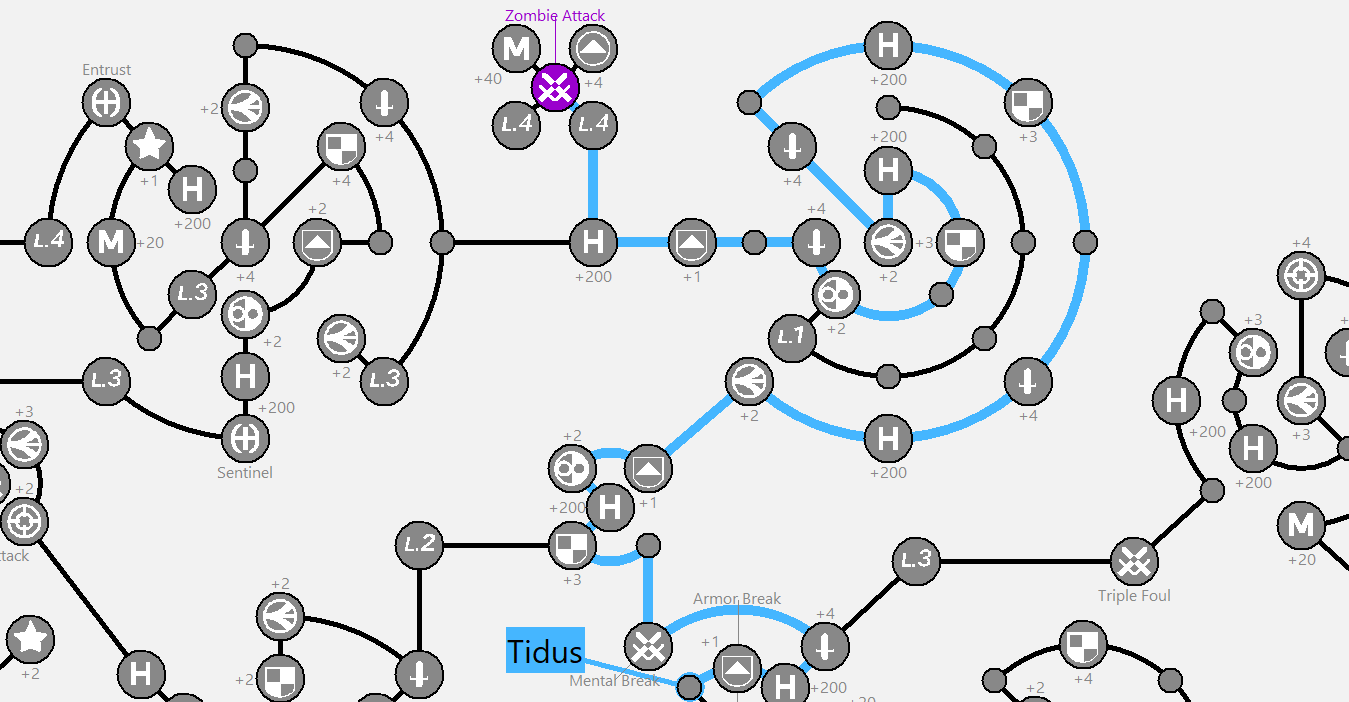
\includegraphics[width=.8\columnwidth]{graphics/Tidus_BFA}
            \rikkuf If no \od, use Skill Sphere to learn Armor Break $\uparrow$
        \end{itemize}
    \end{multicols}
\end{spheregrid}
\colstart
    \begin{equip}
        \begin{itemize}
            \item \textit{If you got a \lulu/\kimahri/\wakka/\rikku\ Zombie Strike weapon:}
            \begin{itemize}
                \item Equip Zombie Strike Weapon
            \end{itemize}
        \end{itemize}
    \end{equip}
    \begin{enumerate}[resume]
        \item Walk up to Jecht, \cs[4:30]
    \end{enumerate}
    \bothvfill\winvfill\lossvfill
    \begin{battle}[180000]{Braska's Final Aeon}
        \begin{itemize}
            \switch{\yuna}{\rikku}
            \rikkuf \od\ Mix Grenade + HP Sphere or Armor Break
            \tidusf Talk
            \switch{\auron}{\yuna}
            \summon{\bahamut}
            \bahamutf Attack
        \end{itemize}
    \end{battle}
\colend
\begin{enumerate}[resume]
    \item \cs+\skippablefmv[4:00]
\end{enumerate}
\begin{battle}{Possessed Aeons}
    \begin{itemize}
        \item Spare Change as follows:
        \begin{itemize}
            \valeforf \num{20000} Gil
            \ifritf \num{30000} Gil
            \ixionf \num{30000} Gil
            \shivaf \num{30000} Gil
            \bahamutf All remaining Gil
        \end{itemize}
    \end{itemize}
\end{battle}
\begin{enumerate}[resume]
    \item \cs[1:40]
\end{enumerate}
\begin{battle}[99999]{Yu Yevon}
    \begin{itemize}
        \item Zombie Attack:
        \begin{itemize}
            \yunaf Defend
            \tidusf Zombie Attack
        \end{itemize}
        \item \yuna\ Zombie Strike Weapon:
        \begin{itemize}
            \yunaf Switch Weapon
            \tidusf Switch Weapon
            \yunaf Attack
        \end{itemize}
        \item \tidus\ Zombie Strike Weapon:
        \begin{itemize}
            \yunaf Defend
            \tidusf Change Weapon
            \tidusf Attack
        \end{itemize}
        \item \rikku\ Zombie Strike Weapon:
        \begin{itemize}
            \yunaf Defend
            \tidusf Haste \rikku
            \yunaf Change Weapon
            \rikkuf Attack
        \end{itemize}
        \item \auron\ Zombie Strike Weapon:
        \begin{itemize}
            \switch{\yuna}{\auron}
            \auronf Change Weapon
            \tidusf Defend
            \auronf Attack
        \end{itemize}
        \item Anyone Else Zombie Strike Weapon:
        \begin{itemize}
            \switch{\yuna}{character with Zombie Strike Weapon}
            \item That Character: Attack
        \end{itemize}
        \item Anyone: Phoenix Down Yu Yevon
    \end{itemize}
\end{battle}
\bothvfill
\colstart
\colend

\end{document}